\appendix
\chapter{Manual de Usuario}
\section{Registro e ingreso de cuentas de usuarios}

Para el ingreso de cuentas de usuarios  se tiene el siguiente formulario para todos los usuarios, donde es necesario que se introduzca el nombre de usuario registrado y la contraseña del mismo. La página de ingreso se muestra a continuación:\\

\begin{figure}[h!]
	\centering
	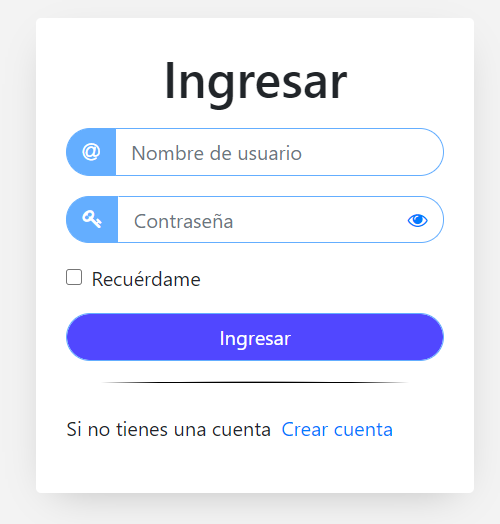
\includegraphics[width=7cm]{./chapters/img/login.png}
	
	\label{fig:login}
	\caption{Login}
\end{figure}

En caso de que las credenciales del usuario sean correctas esta página redireccionará a la página de inicio del sistema que se muestra a continuación:\\

\begin{figure}[h!]
	\centering
	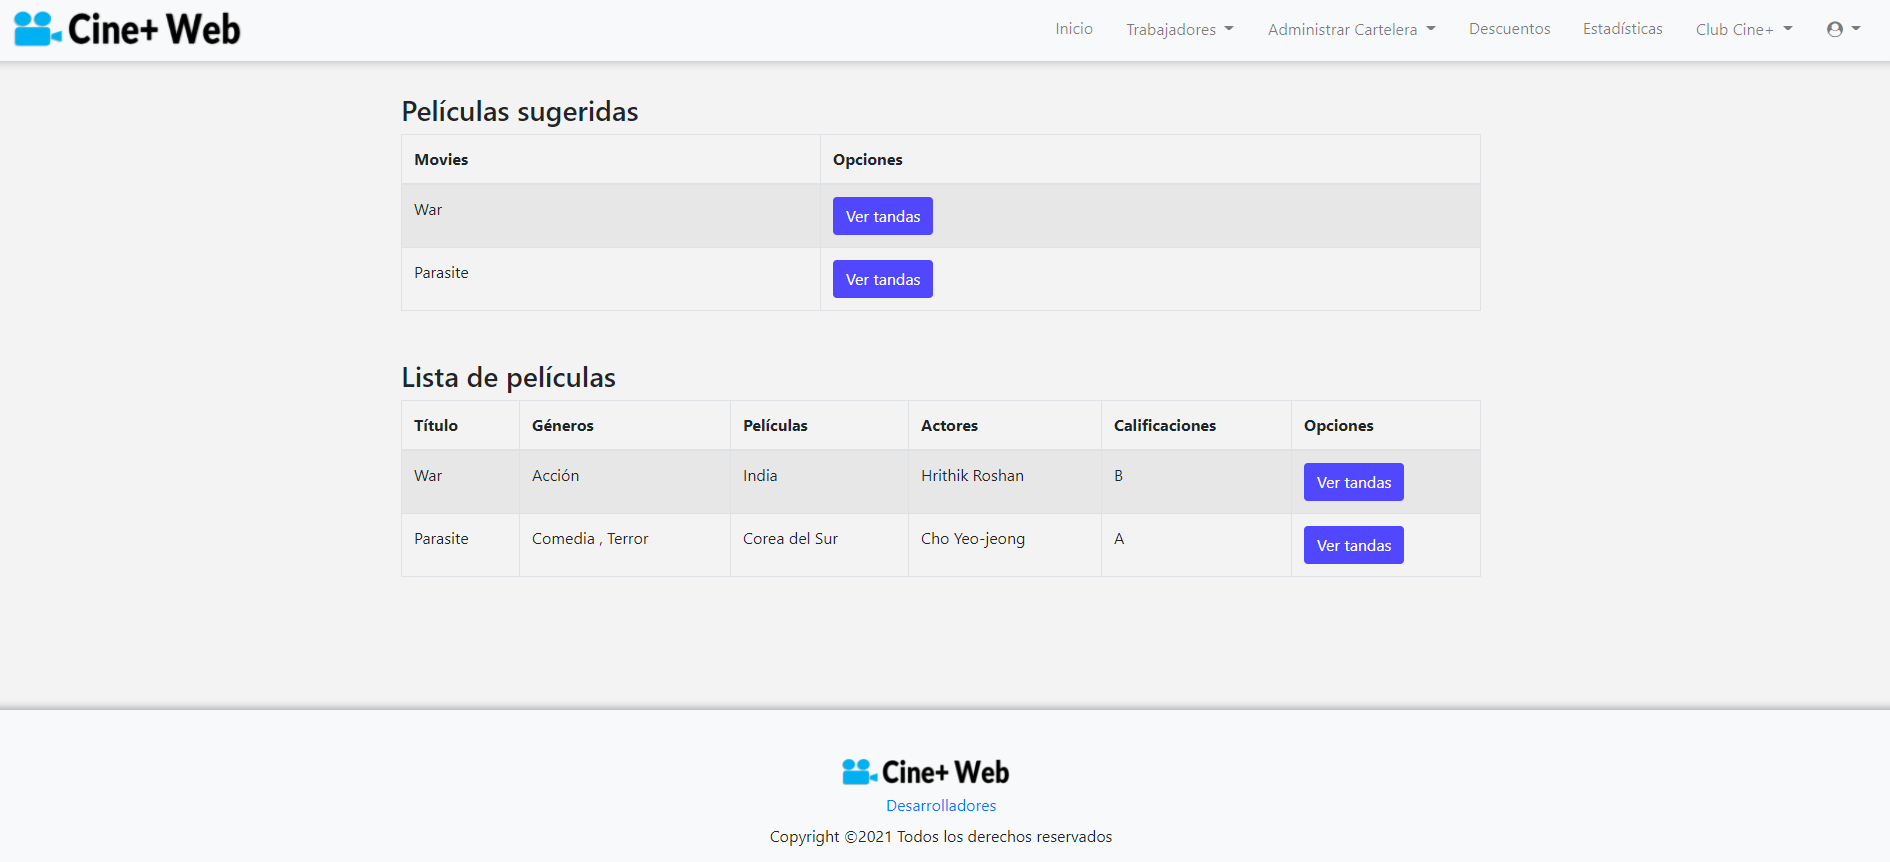
\includegraphics[scale=0.35]{./chapters/img/Index.png}
	
	\label{fig:Index}
	\caption{P\'agina Inicial}
\end{figure}
\newpage

Como se observa en la página de Inicio se tiene una cabecera que está presente en todas las páginas. En la cabecera estará todas las páginas a las que puede acceder un usuario en dependencia de sus permisos.\\

A continuación se presentan las cabeceras de los tres (3) tipos de usuarios:\\

\begin{figure}[h!]
	\centering
	
\includegraphics[scale=0.4]{./chapters/img/header_admin.png}
	
	\label{fig:header_admin}
	\caption{Cabecera Gegerente}
\end{figure}
\begin{figure}[h!]
	\centering
	
\includegraphics[scale=0.4]{./chapters/img/header_taquillero.png}
	
	\label{fig:header_taquillero}
	\caption{Cabecera Taquillero}
\end{figure}
\begin{figure}[h!]
	\centering
	
\includegraphics[scale=0.4]{./chapters/img/header_client.png}
	
	\label{fig:header_client}
	\caption{Cabecera Cliente}
\end{figure}


Para el registro de usuarios se tiene el siguiente formulario accesible desde la cabecera de los usuarios que no están autenticados.
\newpage

\begin{figure}[h!]
	\centering
	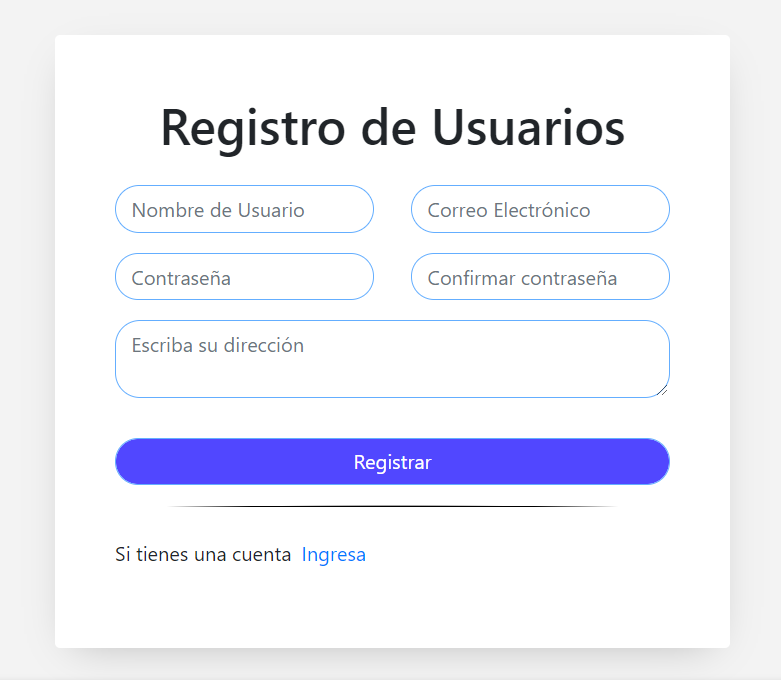
\includegraphics[scale=0.4]{./chapters/img/register.png}
	
	\label{fig:register}
	\caption{Registro}
\end{figure}

Los gerentes son los que est\'an facultados para la designación de nuevos taquilleros y gerentes. Para ello se cuenta con un formulario similar al de registro de usuarios accesible desde \verb|Trabajadores|, opci\'on \verb|Gerentes| y \verb|Taquilleros| disponible en la cabecera de los usuarios con el rol de gerente.\\

Los taquilleros tiene como tarea la venta de entrada en taquilla y la gestion de cuentas de socio.

\subsection{Gestión de Cartelera}

Todas las opciones referentes a la gestión de cartelera est\'an disponibles en las cabeceras en la pesta\~na \verb*|Administar| \verb*|Cartelera|.\\

\begin{figure}[h!]
	\centering
	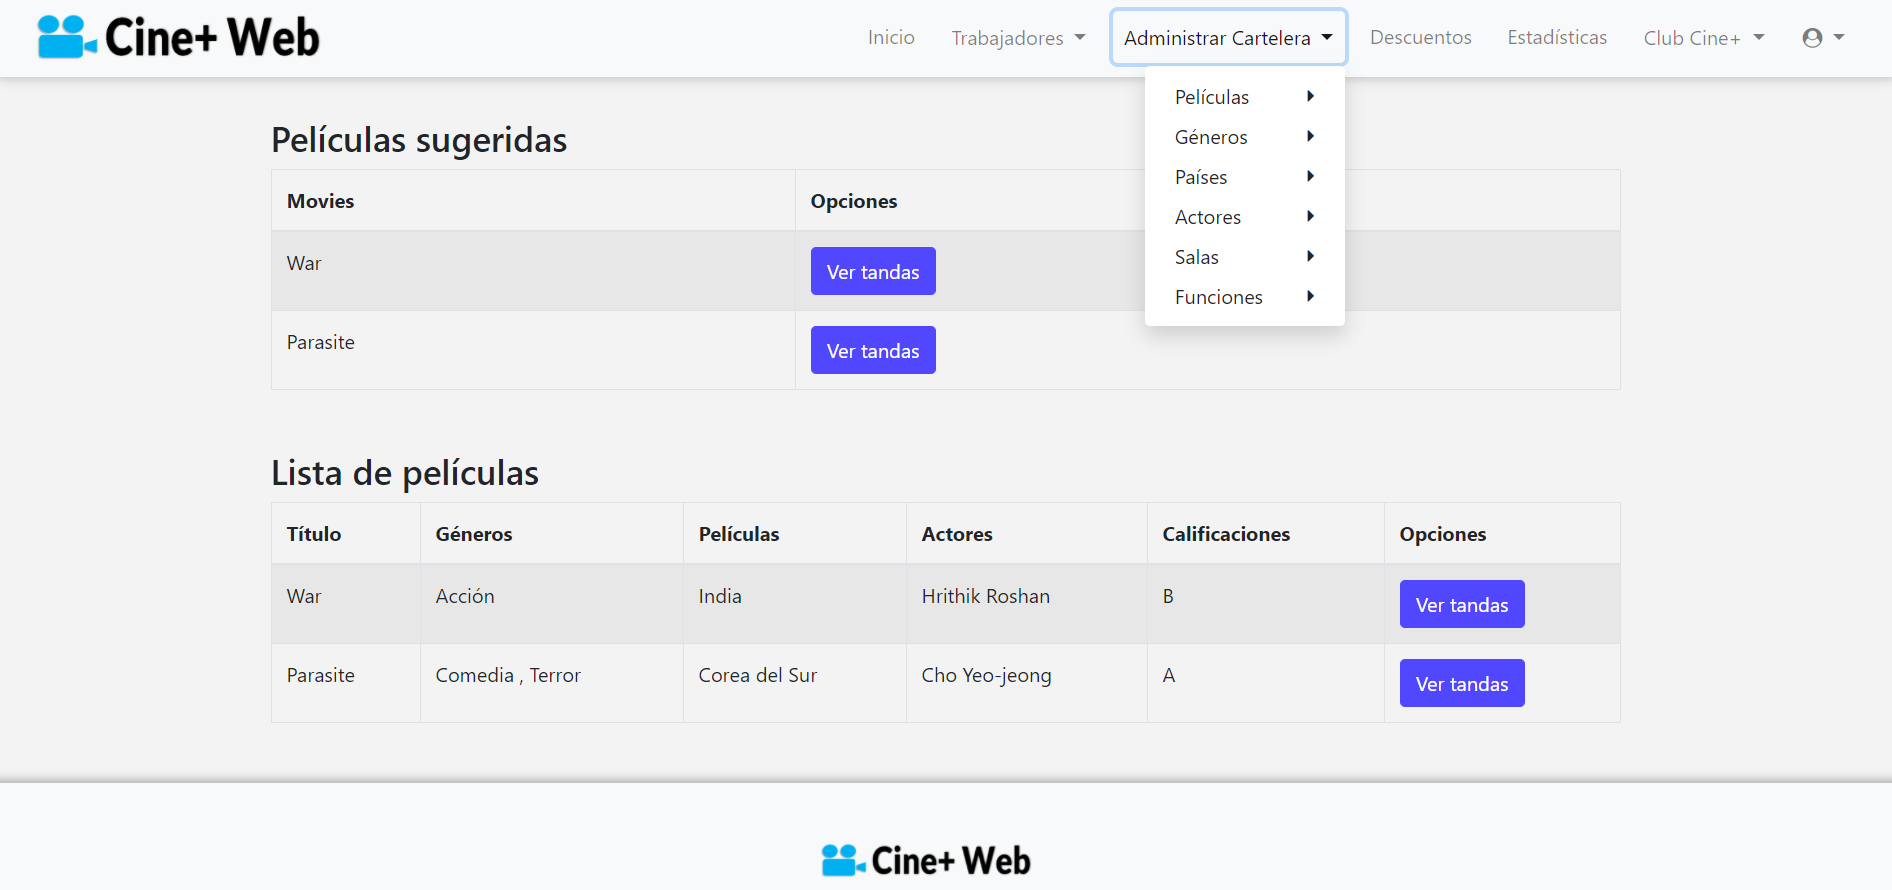
\includegraphics[scale=0.35]{./chapters/img/cartelera.png}
	
	\label{fig:cartelera}
	\caption{Administrar Cartelera}
	
\end{figure}

\subsubsection{Gestor de Pel\'iculas}
La opci\'on referente a la gesti\'on de pel\'iculas es accesible desde la pesta\~na \verb*|Administar| \verb*|Cartelera|. Al hacer click se despliegan dos opciones referentes a pel\'iculas como se observa en la siguiente imagen.

\newpage
\begin{figure}[h!]
	\centering
	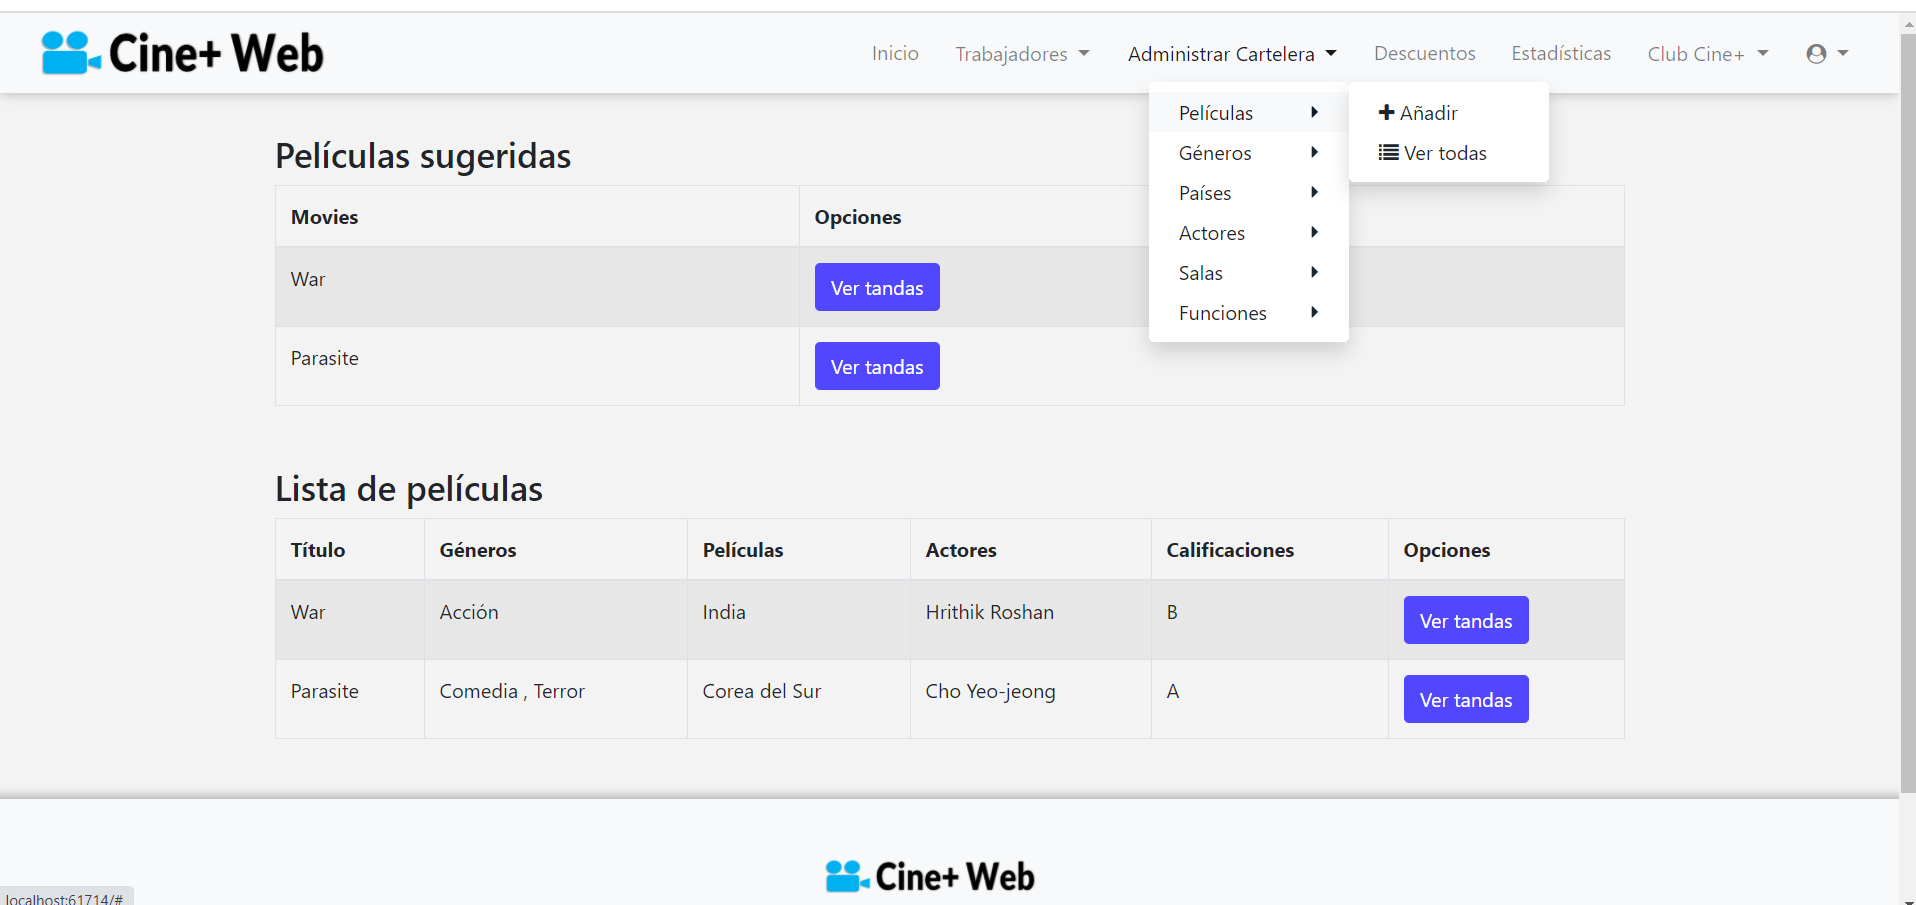
\includegraphics[scale=0.35]{./chapters/img/movie_option.png}
	
	\label{fig:movie_option}
	\caption{Opciones Gestor Pel\'icula}
	
\end{figure}
La opci\'on \verb*|Ver| \verb*|Todas| carga la p\'agina Movies donde se muestra la tabla de las pel\'iculas registradas en la base de datos y la botones para agregar o eliminar estas.

\begin{figure}[h!]
	\centering
	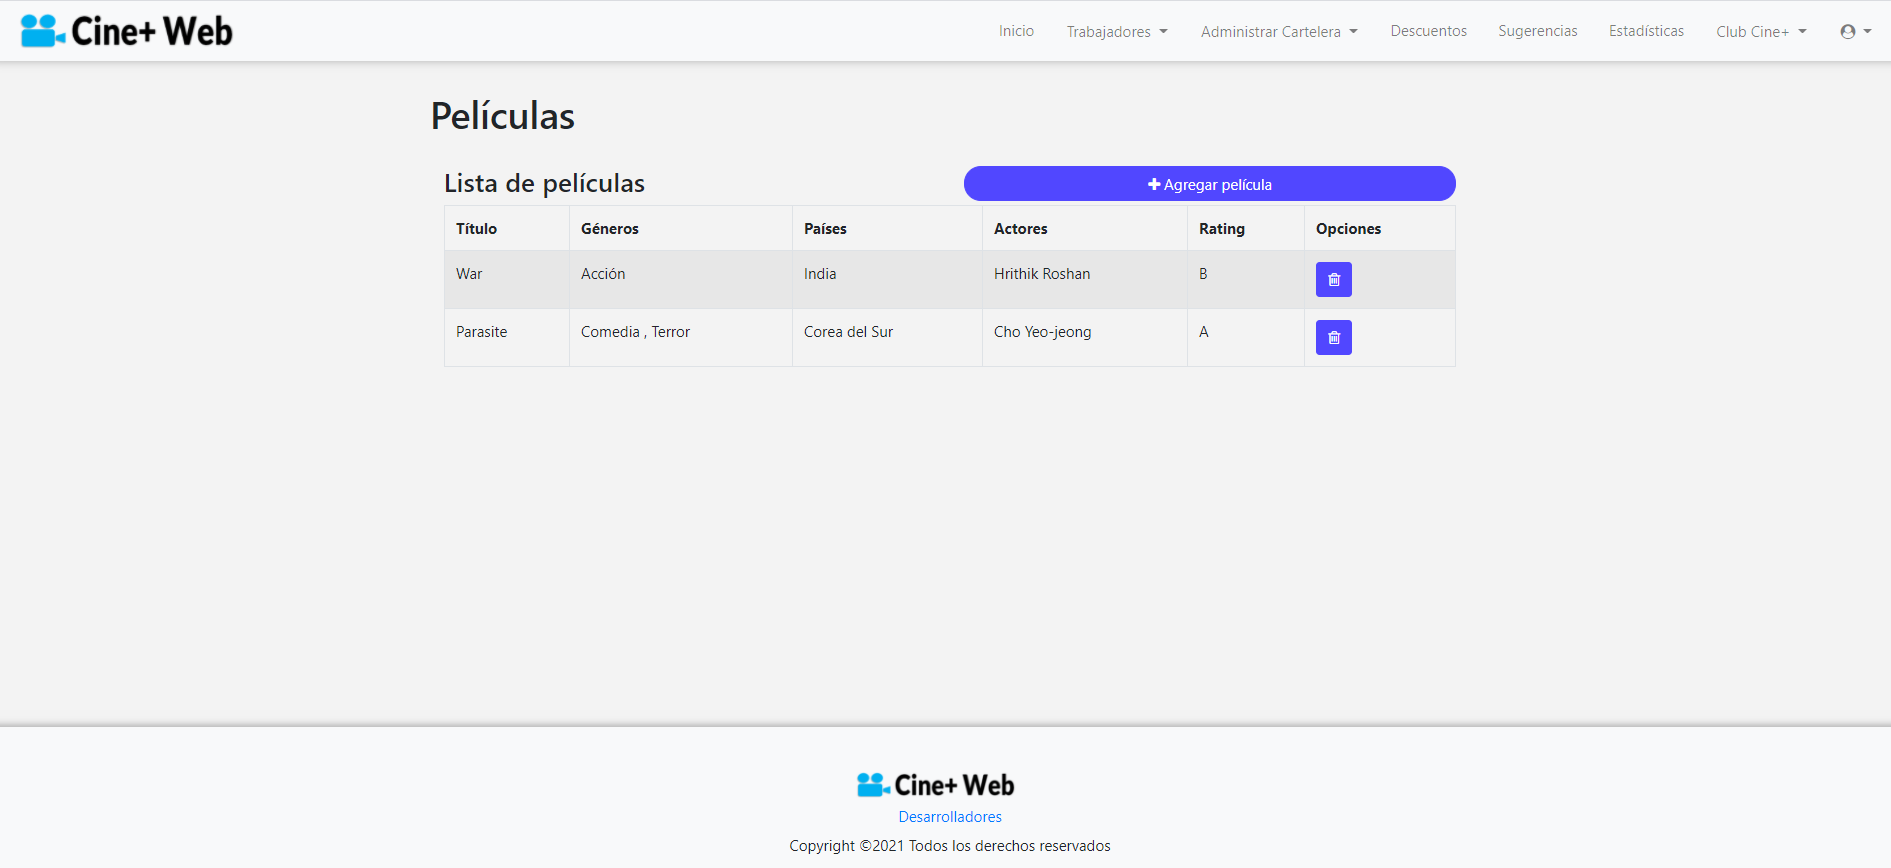
\includegraphics[scale=0.35]{./chapters/img/movies_table.png}
	
	\label{fig:movie_table}
	\caption{P\'agina Movies}
	
\end{figure}

Al agregar una pel\'icula se debe especificar \'el(los) g\'eneros a la que pertenece, la calificaci\'on, pa\'is y los actores que en ella participan as\'i como se observa en la siguiente imagen.
\newpage
\begin{figure}[h!]
	\centering
	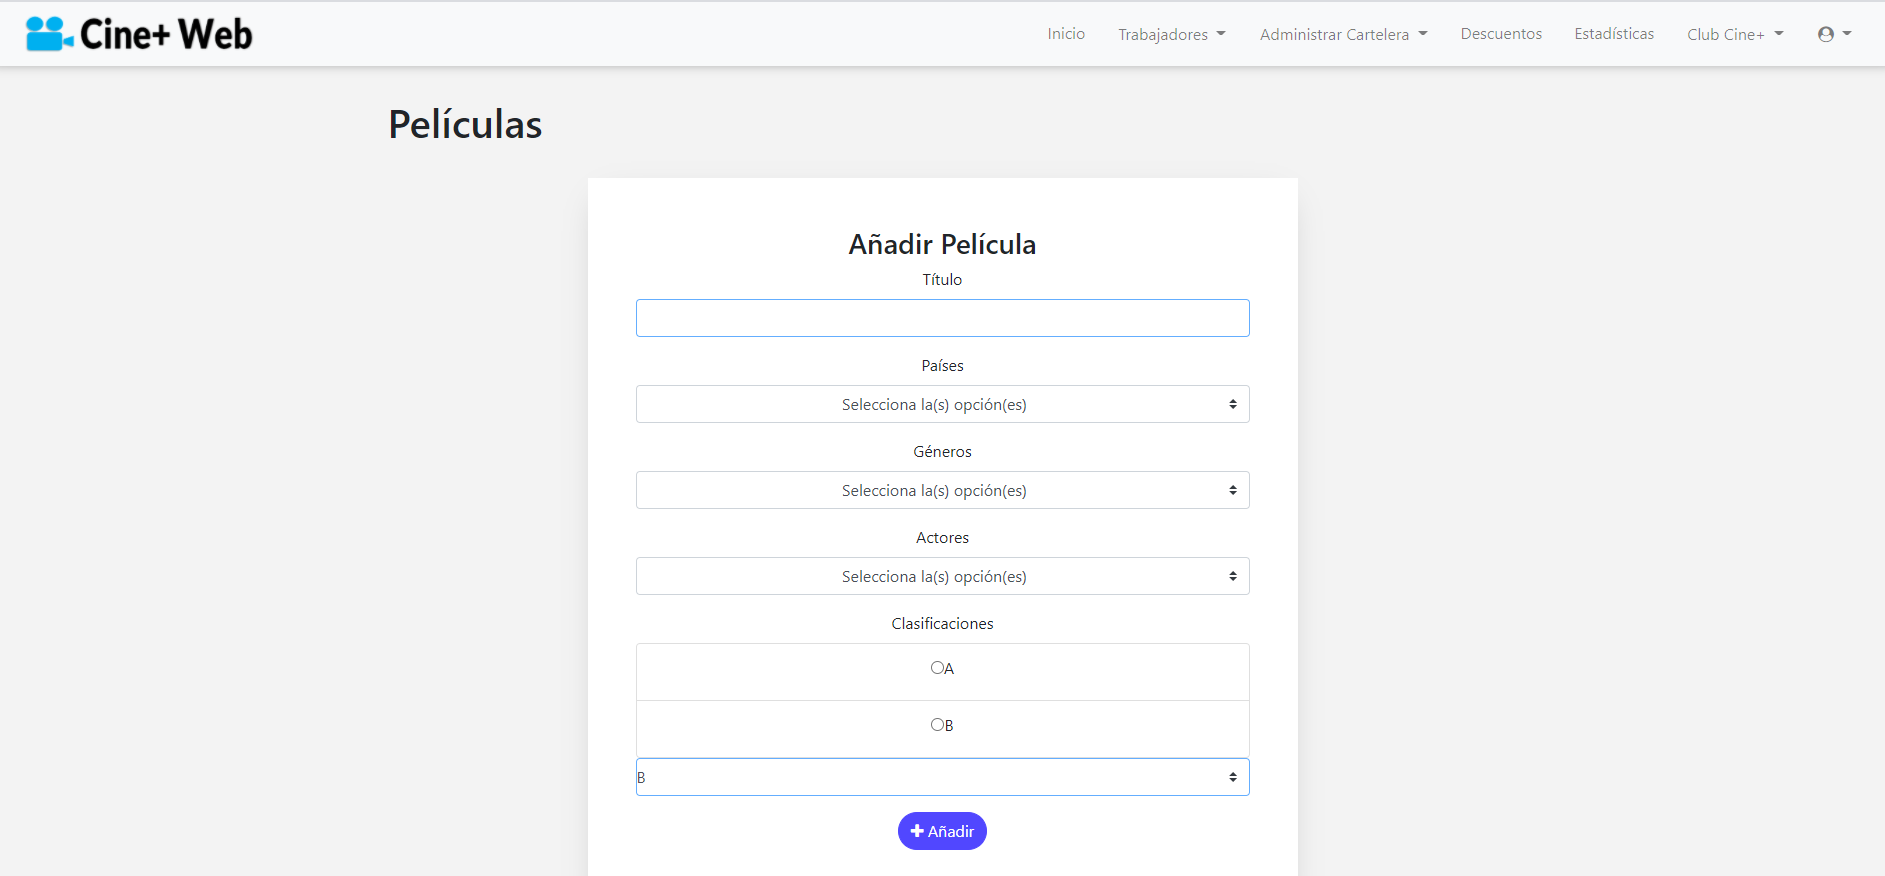
\includegraphics[scale=0.35]{./chapters/img/add_movie.png}
	
	\label{fig:add_movie}
	\caption{Agregar Pel\'icula}
	
\end{figure}

\subsubsection{Gestor de Actores, Pa\'ises, G\'eneros y Salas }

La informaci\'on relacionada con los actores, pa\'ises, g\'eneros y salas se encuentra representada de forma similar que las pel\'iculas. Para la creaci\'on de estos se debe especificar en el caso de g\'enero y pa\'is, el nombre; para los actores, nombre y apellidos y en el otro caso de las salas la capacidad de estas.

\subsubsection{Gestor de Funciones}
La informaci\'on relacionada con las funciones se encuentra representada de forma similar que las pel\'iculas. Para la creaci\'on de estas se debe especificar la fecha de inicio, finalizaci\'on, la sala, la pel\'icula, precio de entrada y precio de la entrada en puntos como se muestra en la siguiente imagen.

\begin{figure}[h!]
	\centering
	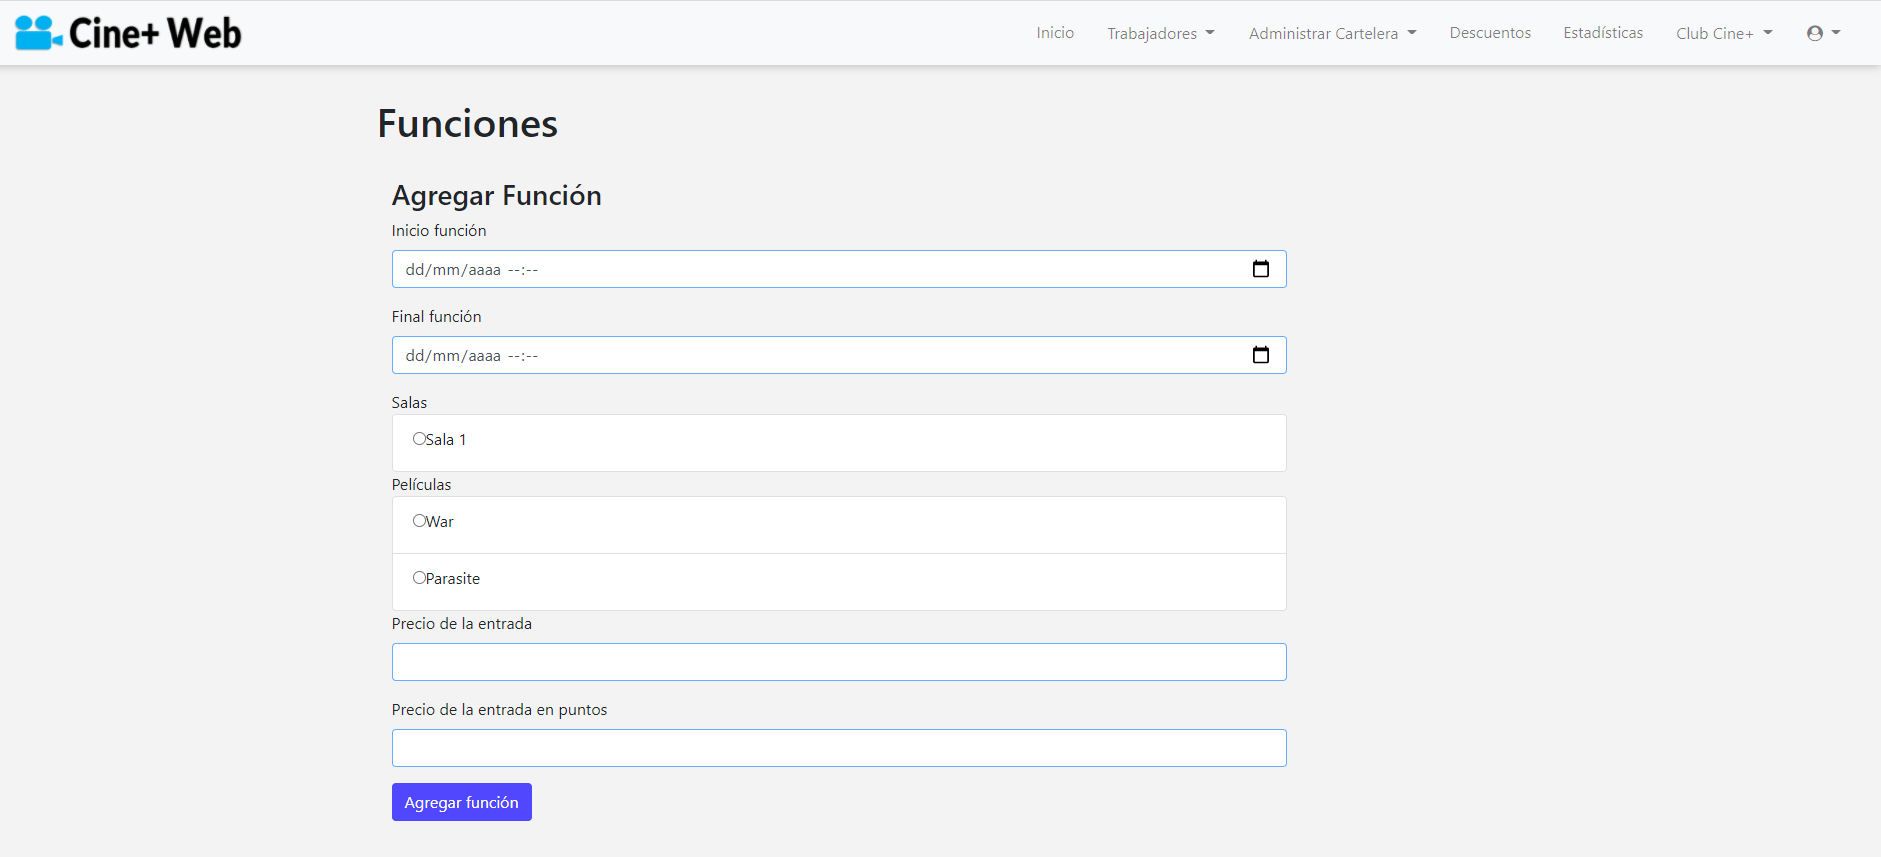
\includegraphics[scale=0.35]{./chapters/img/add_function.png}
	
	\label{fig:add_function}
	\caption{Agregar Funci\'on}
	
\end{figure}

\subsection{Gestor de Socios}
Las opciones referentes a la gesti\'on de socios son accesibles desde la pesta\~na \verb*|Club| \verb*|Cine+| disponible en la cabecera de taquillero y gerente

\begin{figure}[h!]
	\centering
	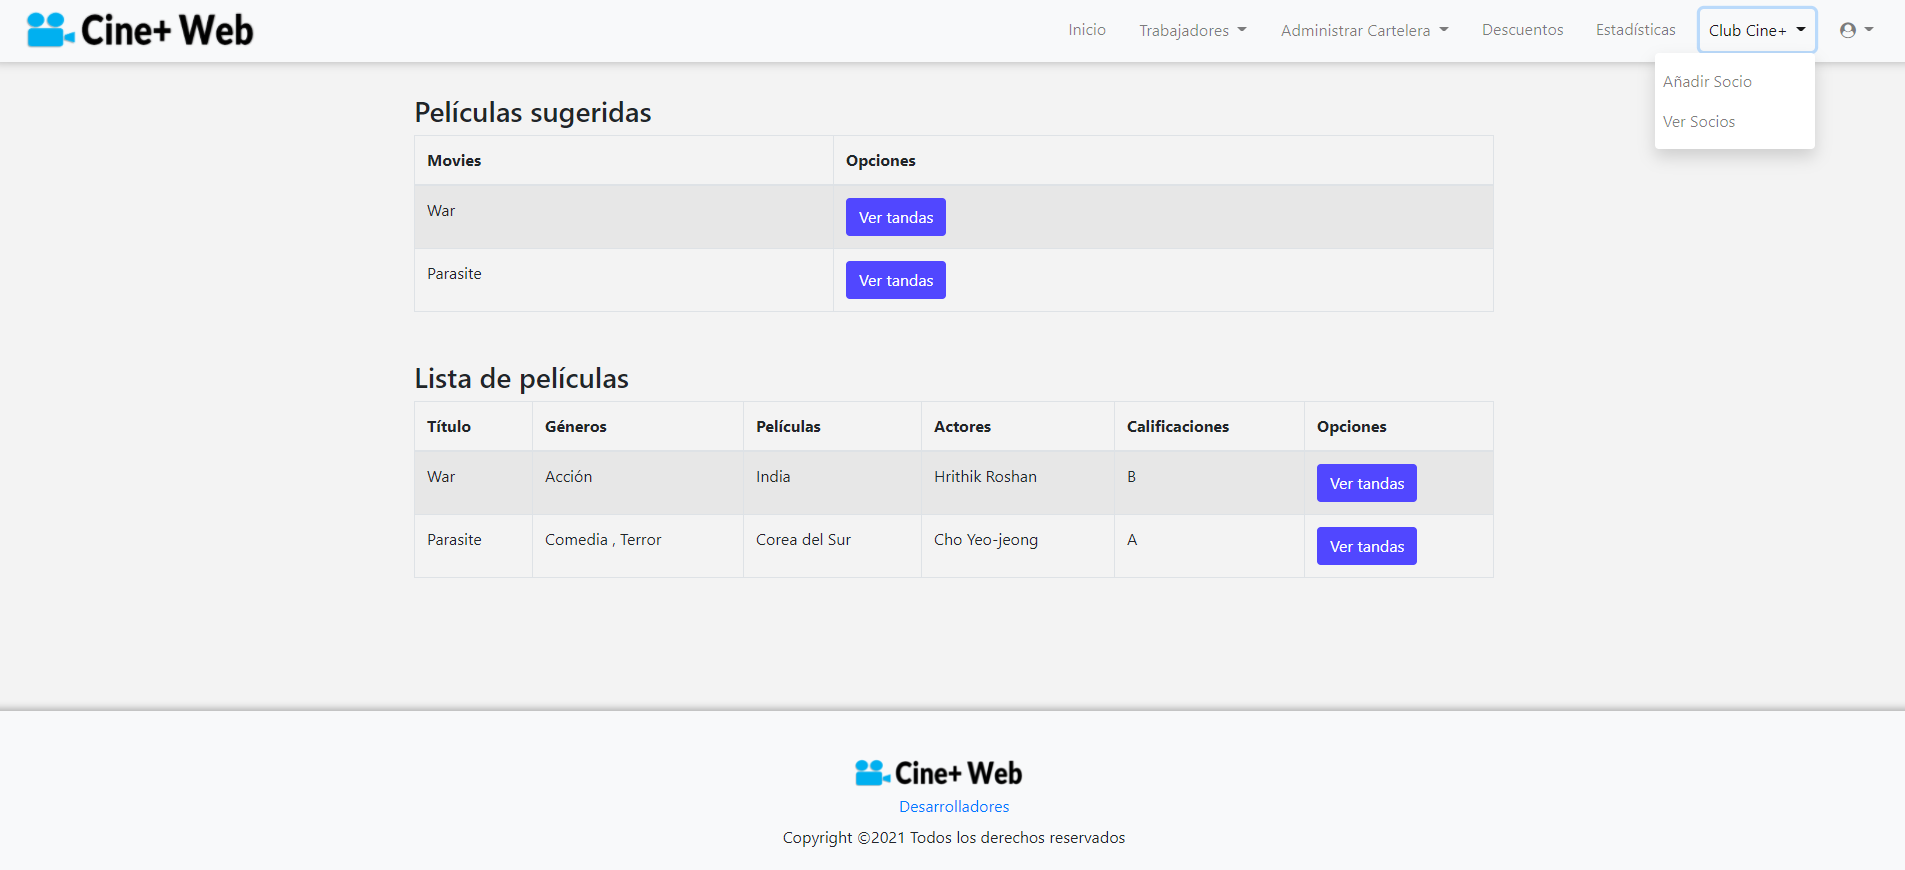
\includegraphics[scale=0.35]{./chapters/img/option_partner.png}
	
	\label{fig:option_partner}
	\caption{Opciones Socios}
	
\end{figure}

La opci\'on \verb*|Ver| \verb*|Socios| direcciona a una p\'agina donde se visualiza el listado de socios registrados y la informaci\'on asociada a estos. De igual manera la opci\'on \verb*|Agregar| \verb*|Socio| permite que los gerentes y taquilleros del cine pueden registrar los socios especificando la informaci\'on asociada a estos en los campos en la p\'agina a la que direcciona como se muestra en la siguiente imagen.

\begin{figure}[h!]
	\centering
	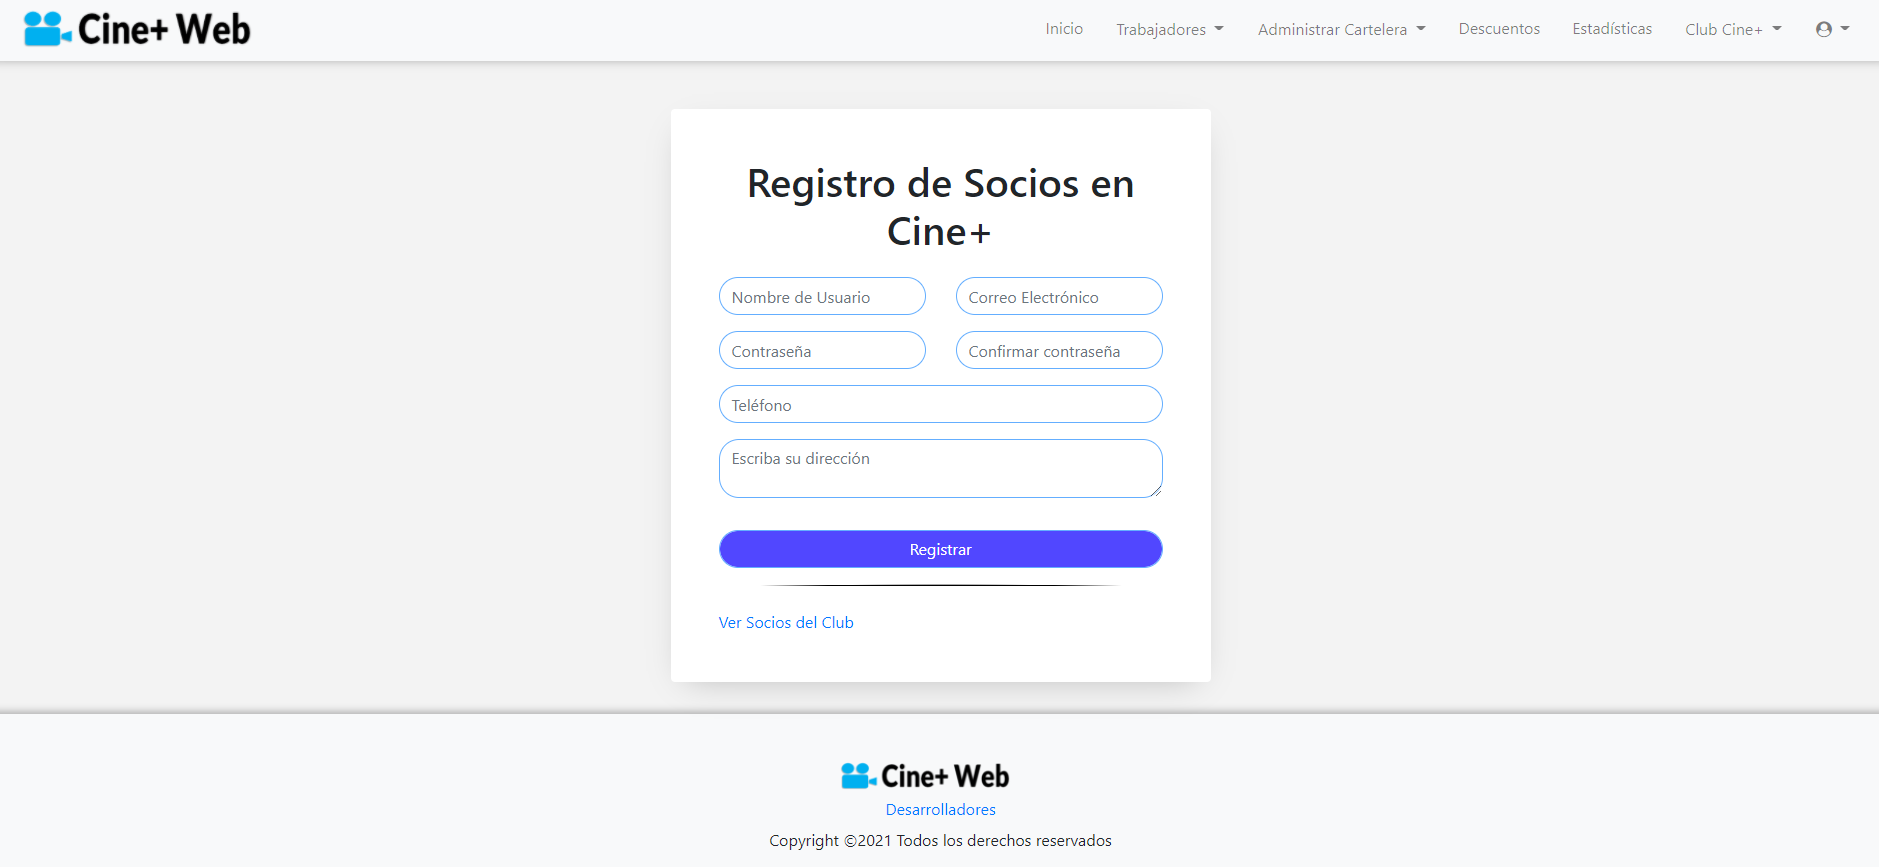
\includegraphics[scale=0.35]{./chapters/img/add_partner.png}
	
	\label{fig:add_partner}
	\caption{Agregar Socio}
	
\end{figure}

\subsection{Gestor de Descuentos}
La pesta\~na \verb*|Descuentos| disponible en la cabecera direcciona a la p\'agina donde se visualiza la lista de descuentos registradas; estas pueden ser editadas o eliminadas. El bot\'on \verb*|Agregar| \verb*|Descuento| redirecciona a la p\'agina donde los gerentes crean estos descuentos especificando los campos nombre y la cantidad de dinero descontado como se muestra en la siguiente imagen.

\begin{figure}[h!]
	\centering
	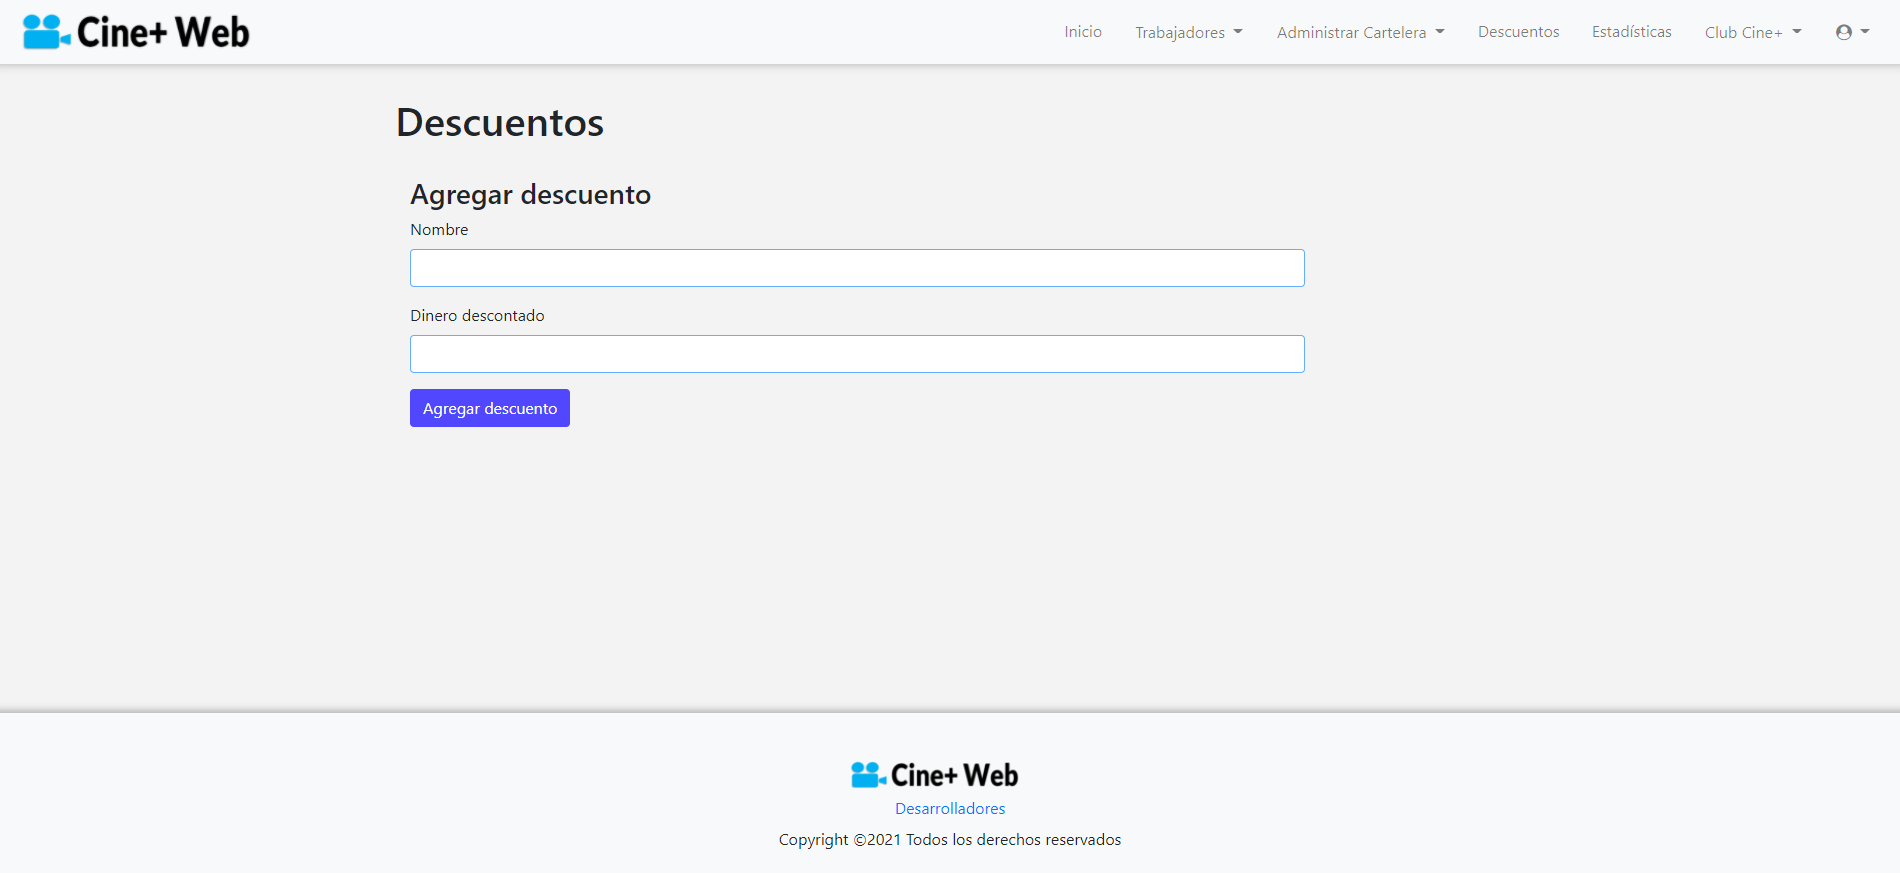
\includegraphics[scale=0.35]{./chapters/img/add_discount.png}
	
	\label{fig:add_discount}
	\caption{Agregar Descuento}
	
\end{figure}



\subsection{Gestor de Trabajadores}
La pesta\~na \verb*|Trabajadores| disponible desde la cabecera de los gerentes despliega dos opciones, la primera \verb*|Taquilleros| la cual direcciona a una p\'agina donde se muestran la informaci\'on referente a los taquilleros registrados y muestra la opci\'on \verb*|Registrar|  \verb*|Taquillero| con un formulario similar al del registro de usuario.

\begin{figure}[h!]
	\centering
	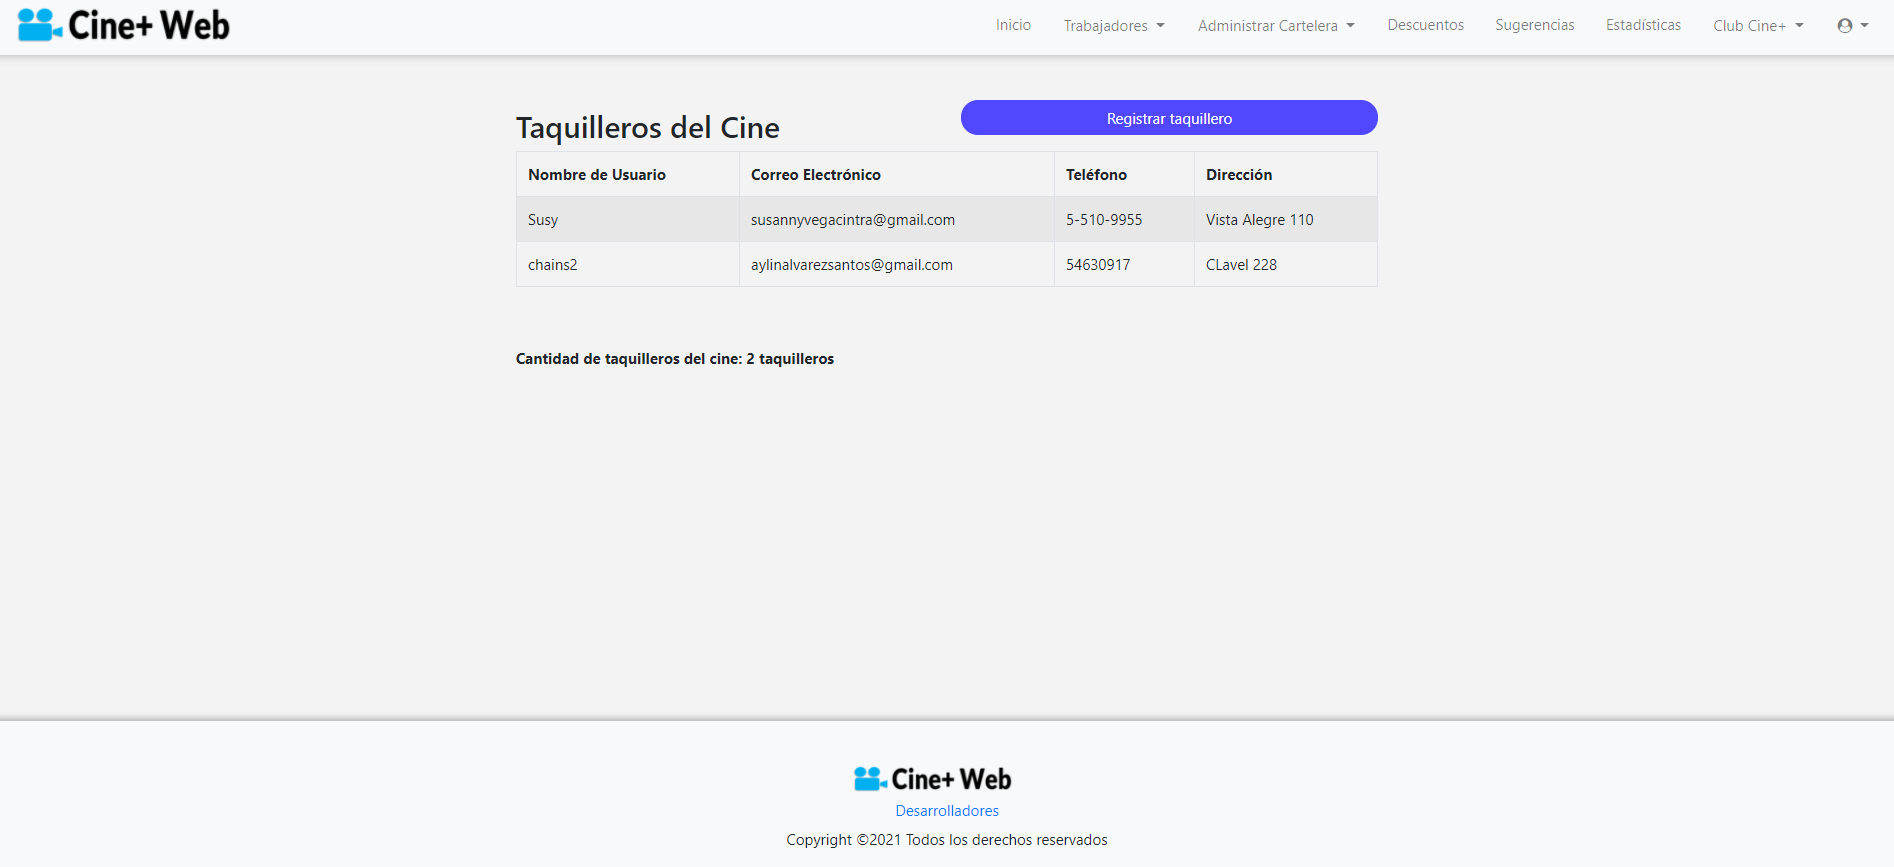
\includegraphics[scale=0.35]{./chapters/img/ver_taquilleros.png}
	
	\label{fig:ver_taquilleros}
	\caption{Taquilleros}
	
\end{figure}

La segunda opci\'on \verb*|Gerentes| direcciona a una p\'agina donde se muestran la informaci\'on referente a los gerentes registrados y muestra la opci\'on \verb*|Registrar|  \verb*|Gerente| con un formulario similar al del registro de usuario.
\newpage
\begin{figure}[h!]
	\centering
	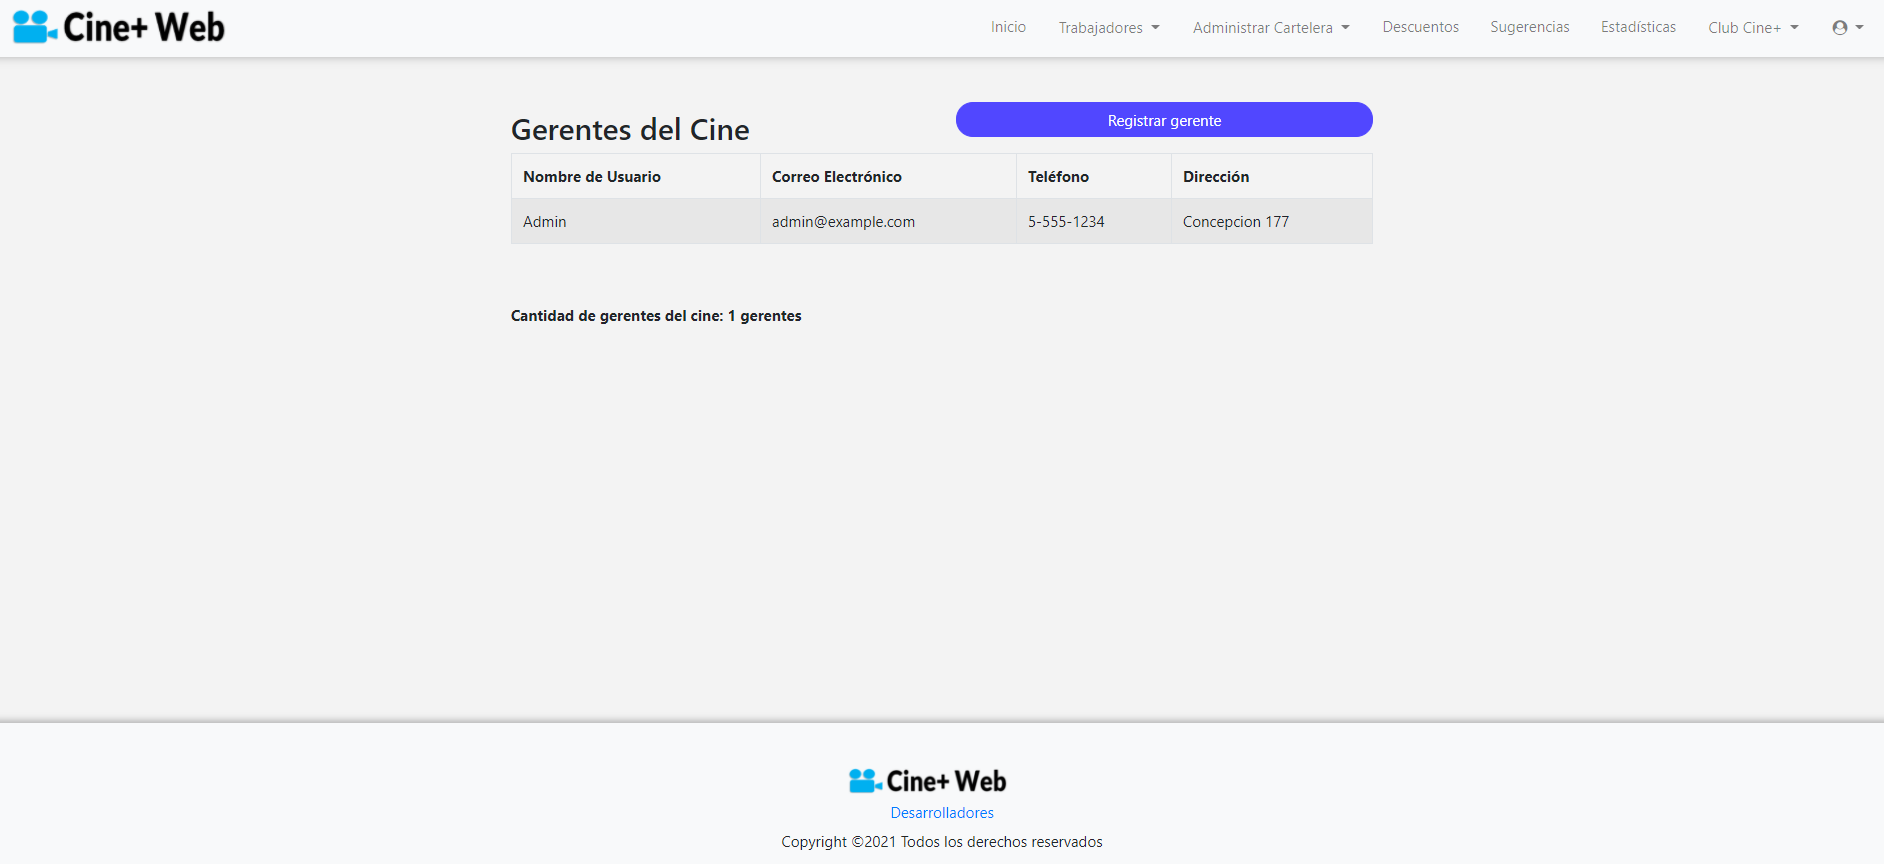
\includegraphics[scale=0.35]{./chapters/img/ver_gerentes.png}
	
	\label{fig:ver_gerentes}
	\caption{Gerentes}
	
\end{figure}

\subsection{Sugerencias}
Esta opci\'on es accesible desde las cabecera de los gerentes, esta direcciona a una p\'agina donde se muestran los criterios a aplicar en la sugerencia de pel\'iculas que se muestra en la p\'agina inicial de la aplicaci\'on.

\begin{figure}[h!]
	\centering
	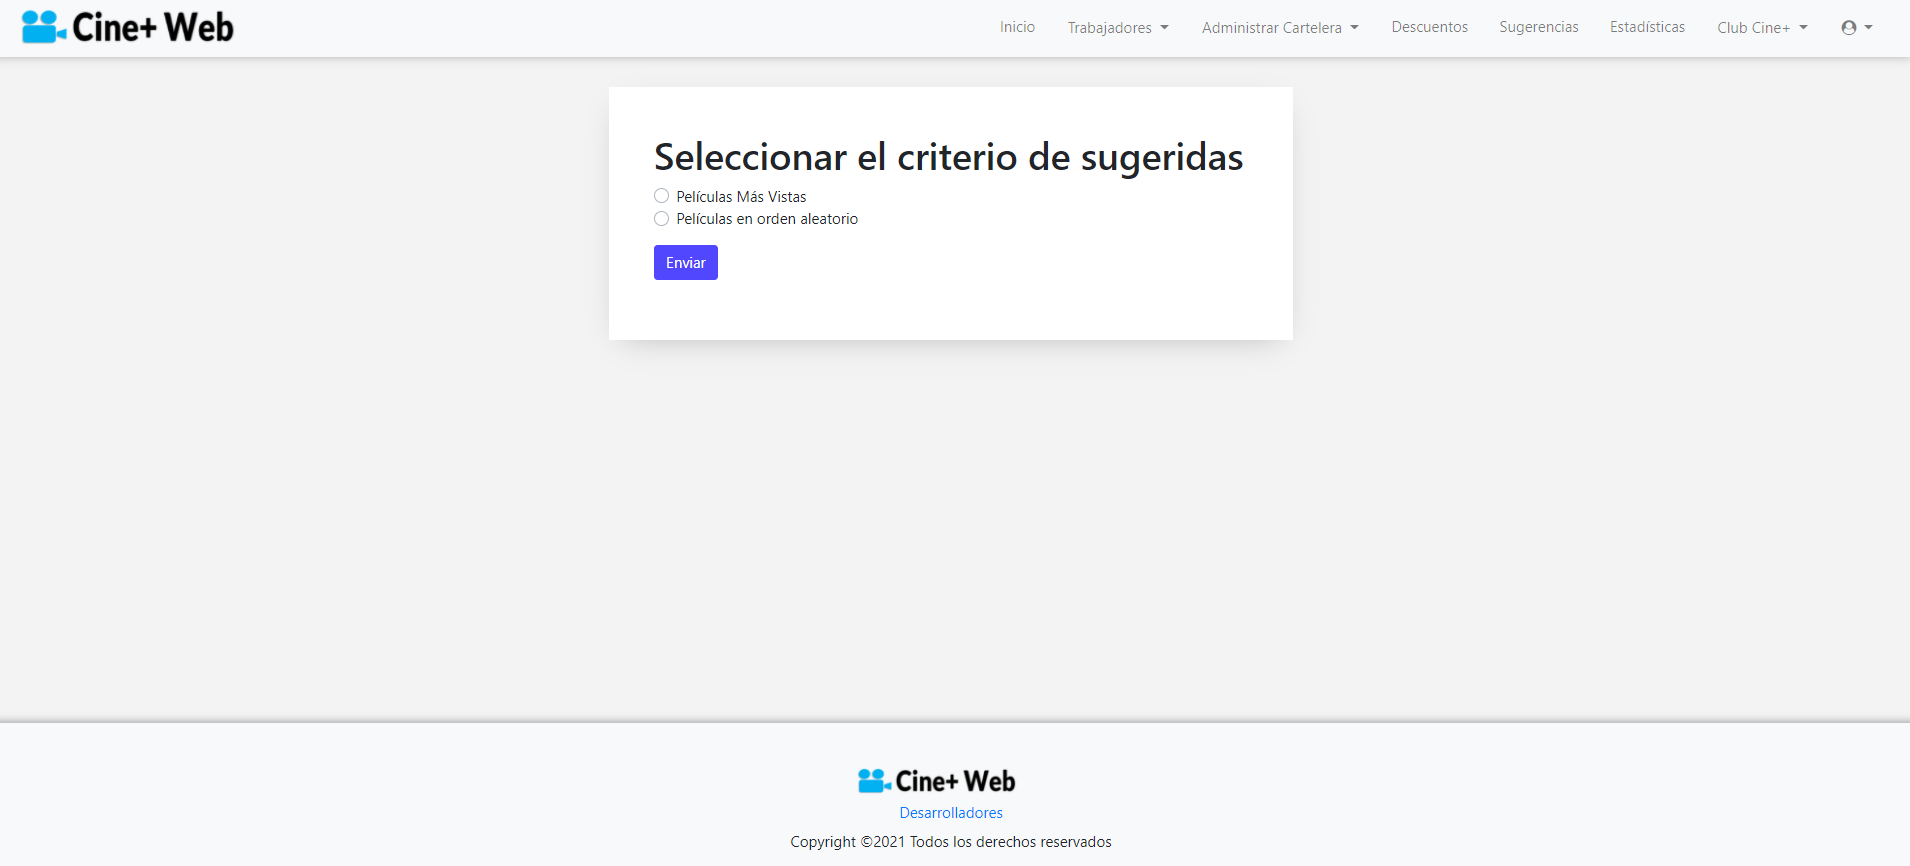
\includegraphics[scale=0.35]{./chapters/img/criteria.png}
	
	\label{fig:criteria}
	\caption{Sugerencias}
	
\end{figure}

\subsection{Estad\'isticas}
Esta opci\'on es accesible desde las cabecera de los gerentes, esta direcciona a una p\'agina donde se muestran las diferentes opciones para la consulta de ventas seg\'un el filtro escogido.
\newpage
\begin{figure}[h!]
	\centering
	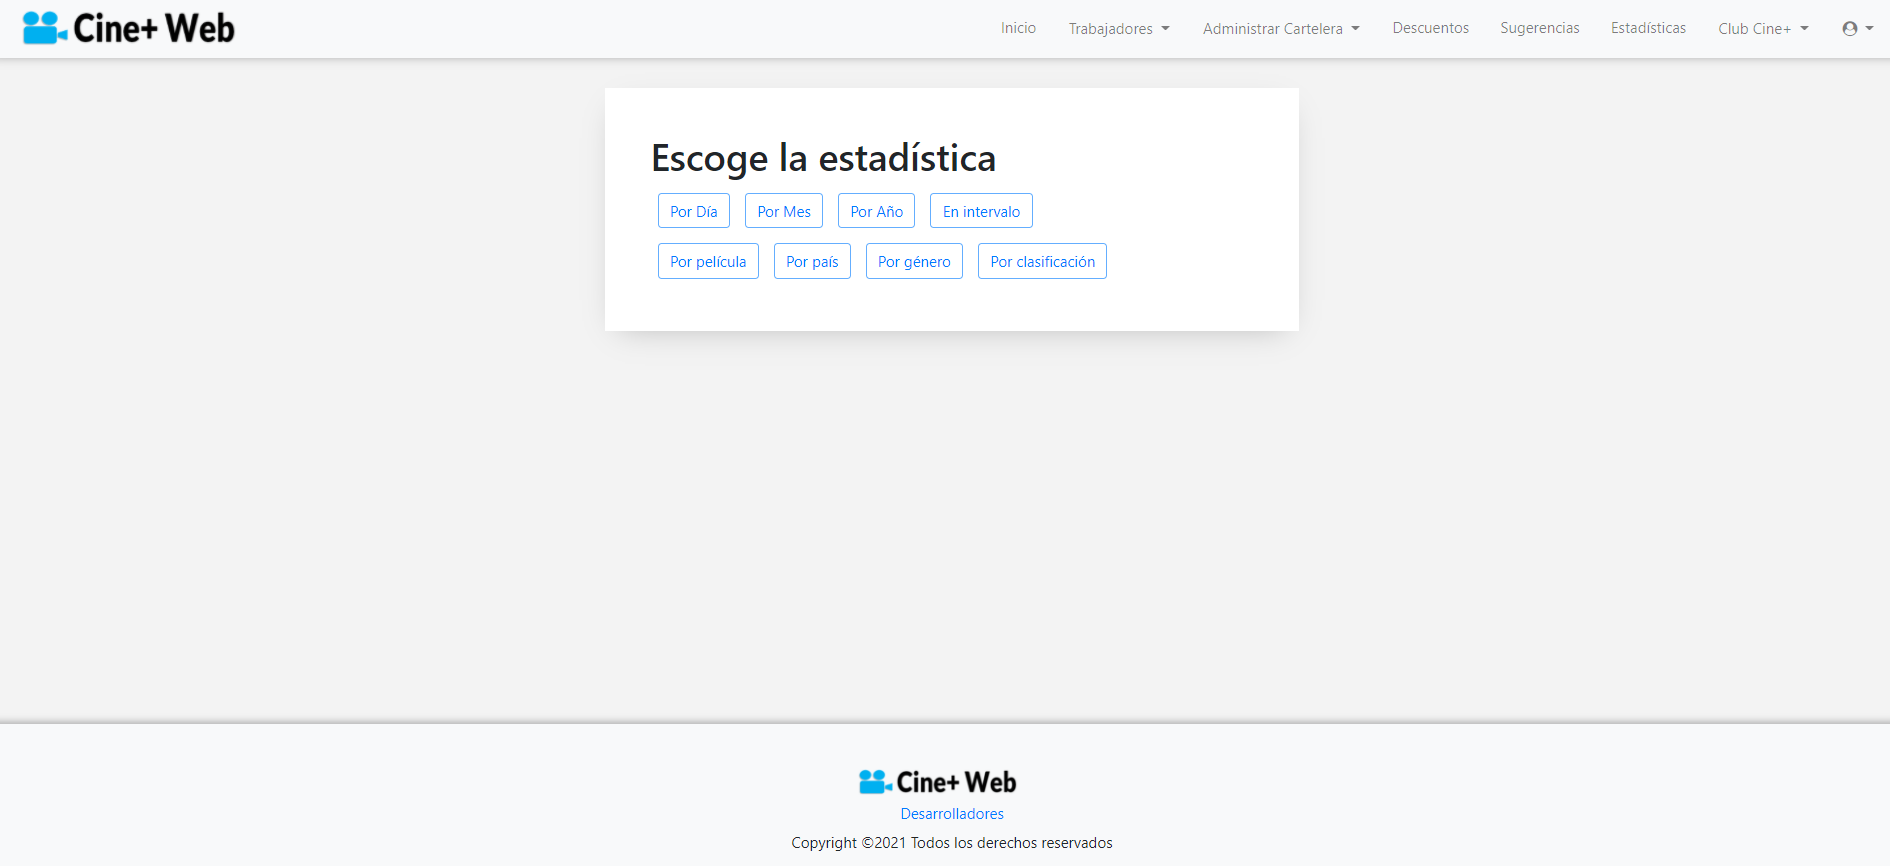
\includegraphics[scale=0.35]{./chapters/img/statistics.png}
	
	\label{fig:statistics}
	\caption{Estad\'isticas}
	
\end{figure}
\subsection{Compra de entradas}
Un usuario logueado o no, puede visualizar las funciones tanto desde la p\'agina inicial accediendo a las tandas desde el bot\'on ubicado en el mismo rengl\'on de la pel\'icula referida como desde la pesta\~na Cartelera disponible en la cabecera para los usuarios clientes, esta \'ultima al hacer click direcciona a la p\'agina donde se muestra el listado de funciones, en cada rengl\'on se muestra una funci\'on y las opciones asociadas a estas.\\

\subsubsection{Paso 1}
En este paso se muestra el campo de C\'odigo de Socio que puede ser especificado en caso del  estar registrado como socio y en el campo el N\'umero de entradas se debe especificar la cantidad de estas, para avanzar se debe hacer click en el bot\'on \verb*|Aceptar|\\

\begin{figure}[h!]
	\centering
	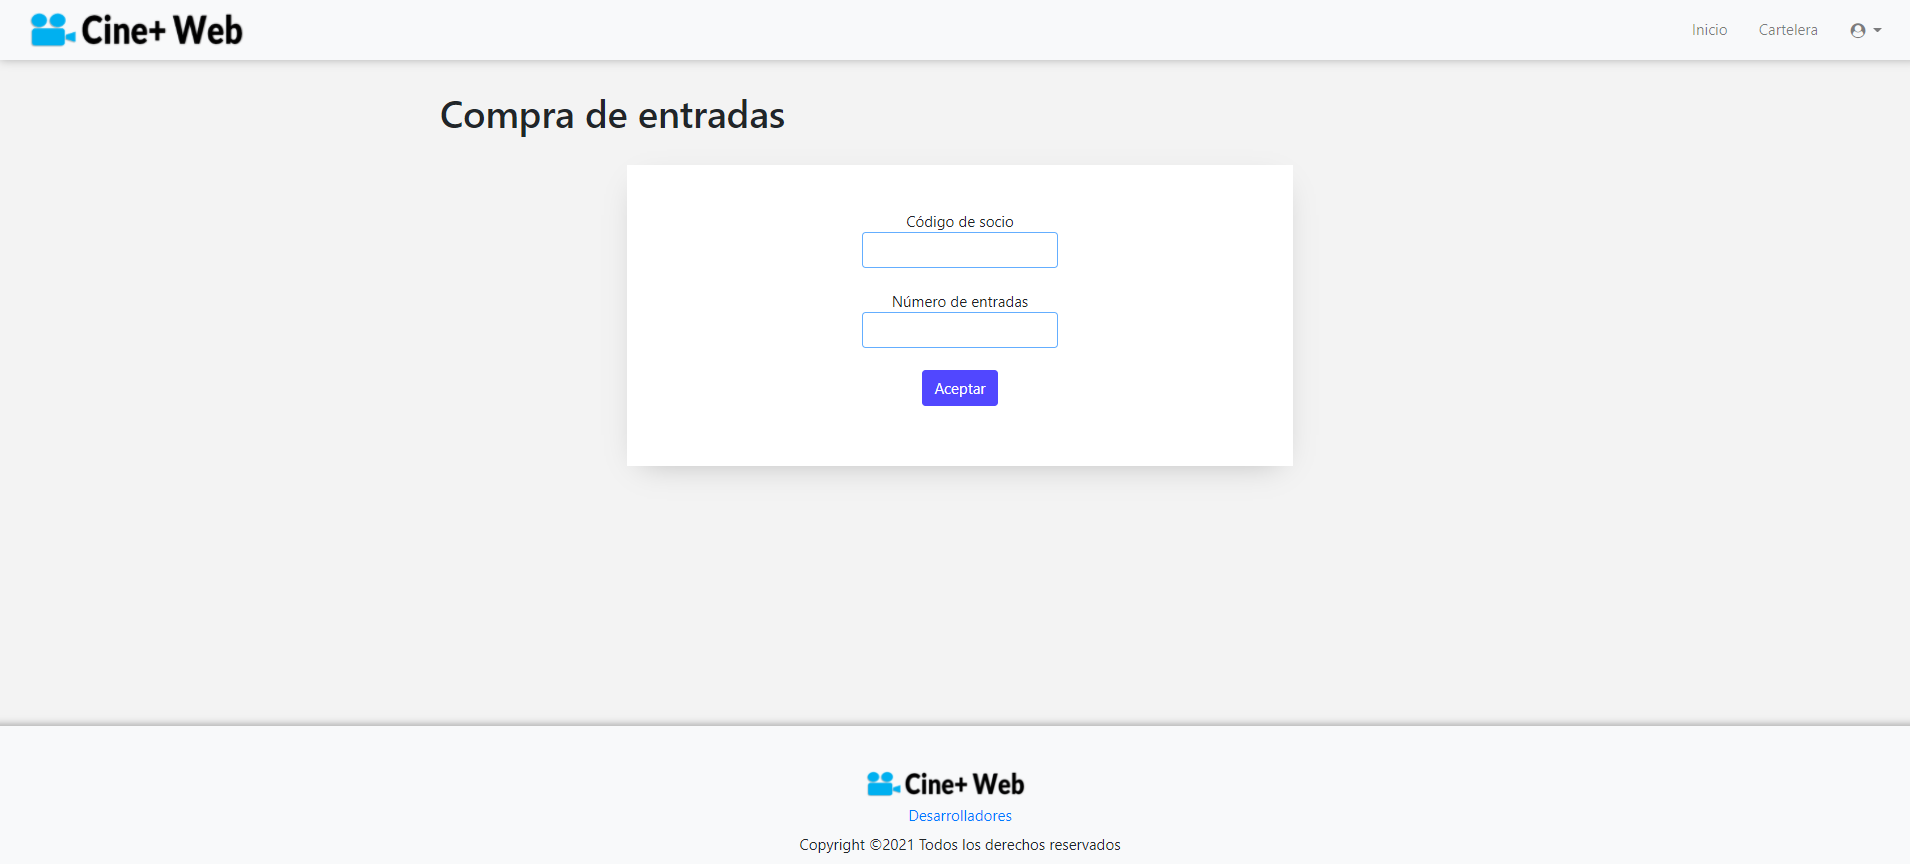
\includegraphics[scale=0.35]{./chapters/img/ticketpurchase1.png}
	
	\label{fig:ticketpurchase1}
	\caption{Compra de entradas}
	
\end{figure}

\subsubsection{Paso 2}
En este paso se muestra las sillas disponibles de la sala donde se puede seleccionar a conveniencia, el sistema autom\'aticamente seleccionar\'a de forma consecutiva en caso de estar disponibles de acuerdo a la cantidad especificada en el paso anterior, para avanzar se debe hacer click en el bot\'on \verb*|Enviar| \verb*|Sillas|.

\begin{figure}[h!]
	\centering
	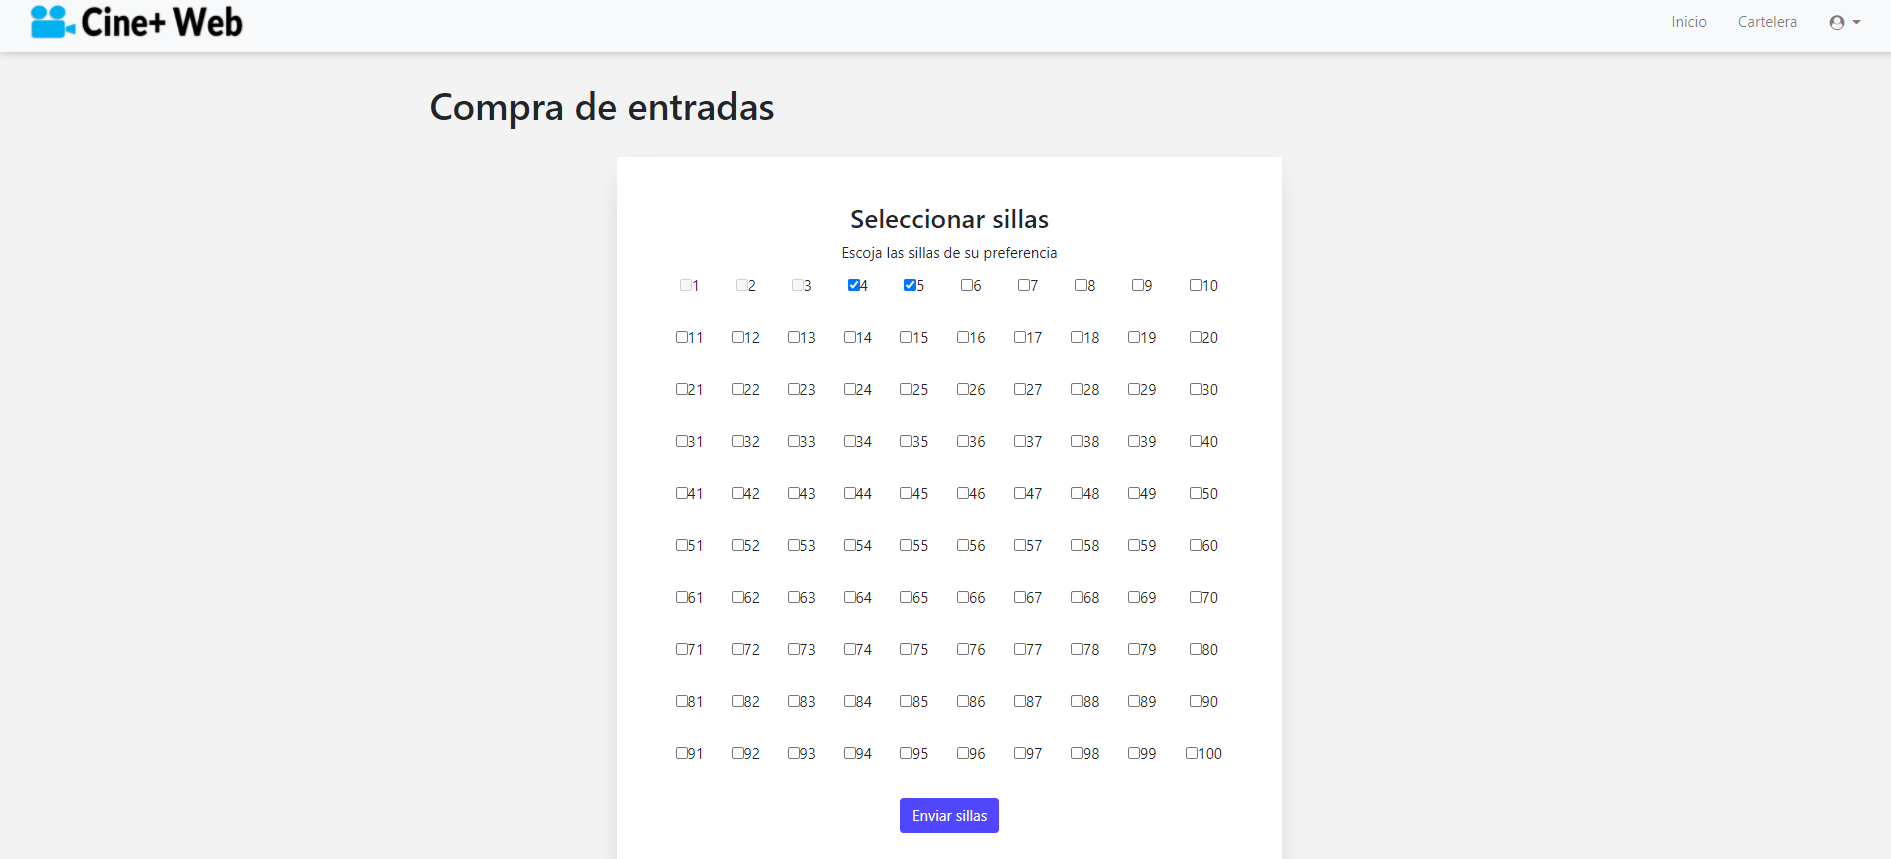
\includegraphics[scale=0.35]{./chapters/img/seat.png}
	
	\label{fig:seats}
	\caption{Seleccionar Sillas}
\end{figure}

\subsubsection{Paso 3}
En este paso se muestra la lista de descuentos disponibles a aplicar para cada silla. En caso que se desee puede especificar por cada silla el descuento a aplicar, luego debe proceder a reservar las silla ya sea la cantidad especificada inicial o una cantidad menor a esta, para avanzar se debe hacer click en el bot\'on \verb*|Pagar|.

\begin{figure}[h!]
	\centering
	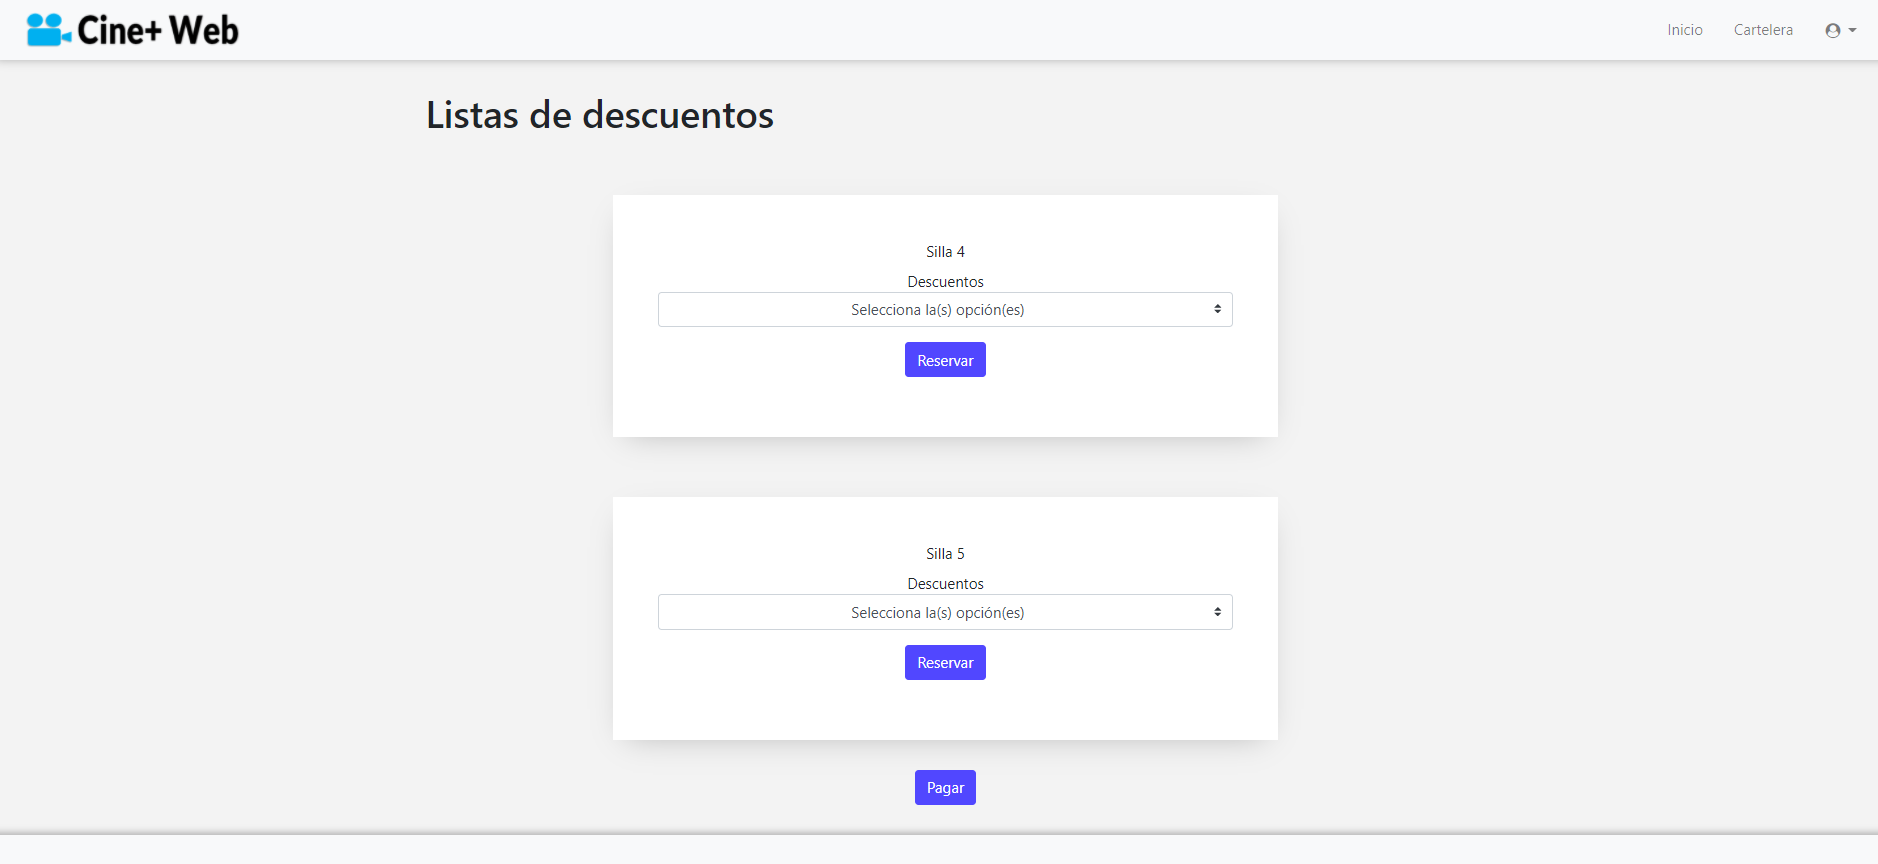
\includegraphics[scale=0.35]{./chapters/img/reserve.png}
	
	\label{fig:reserve}
	\caption{Reservar Sillas}
\end{figure}

\subsubsection{Paso 4}
En este paso se muestra el total a pagar con dinero y con puntos, este \'ultimo aparece en caso de que sea especificado el c\'odigo de socio en el paso 1. Adem\'as aparecen el campo tarjeta de cr\'edito y la opci\'on de pagar con dinero. En caso que se desee pagar con dinero se deber\'a especificar el n\'umero de tarjeta de cr\'edito solo en compras online en el campo correspondiente, en otro caso, se podr\'a pagar con puntos en caso de tener los suficientes para la compra, para esta opci\'on se debe activar la opci\'on  Pagar con Puntos. Para avanzar al pr\'oximo paso se hacer click en el bot\'on \verb*|Pagar|.

\begin{figure}[h!]
	\centering
	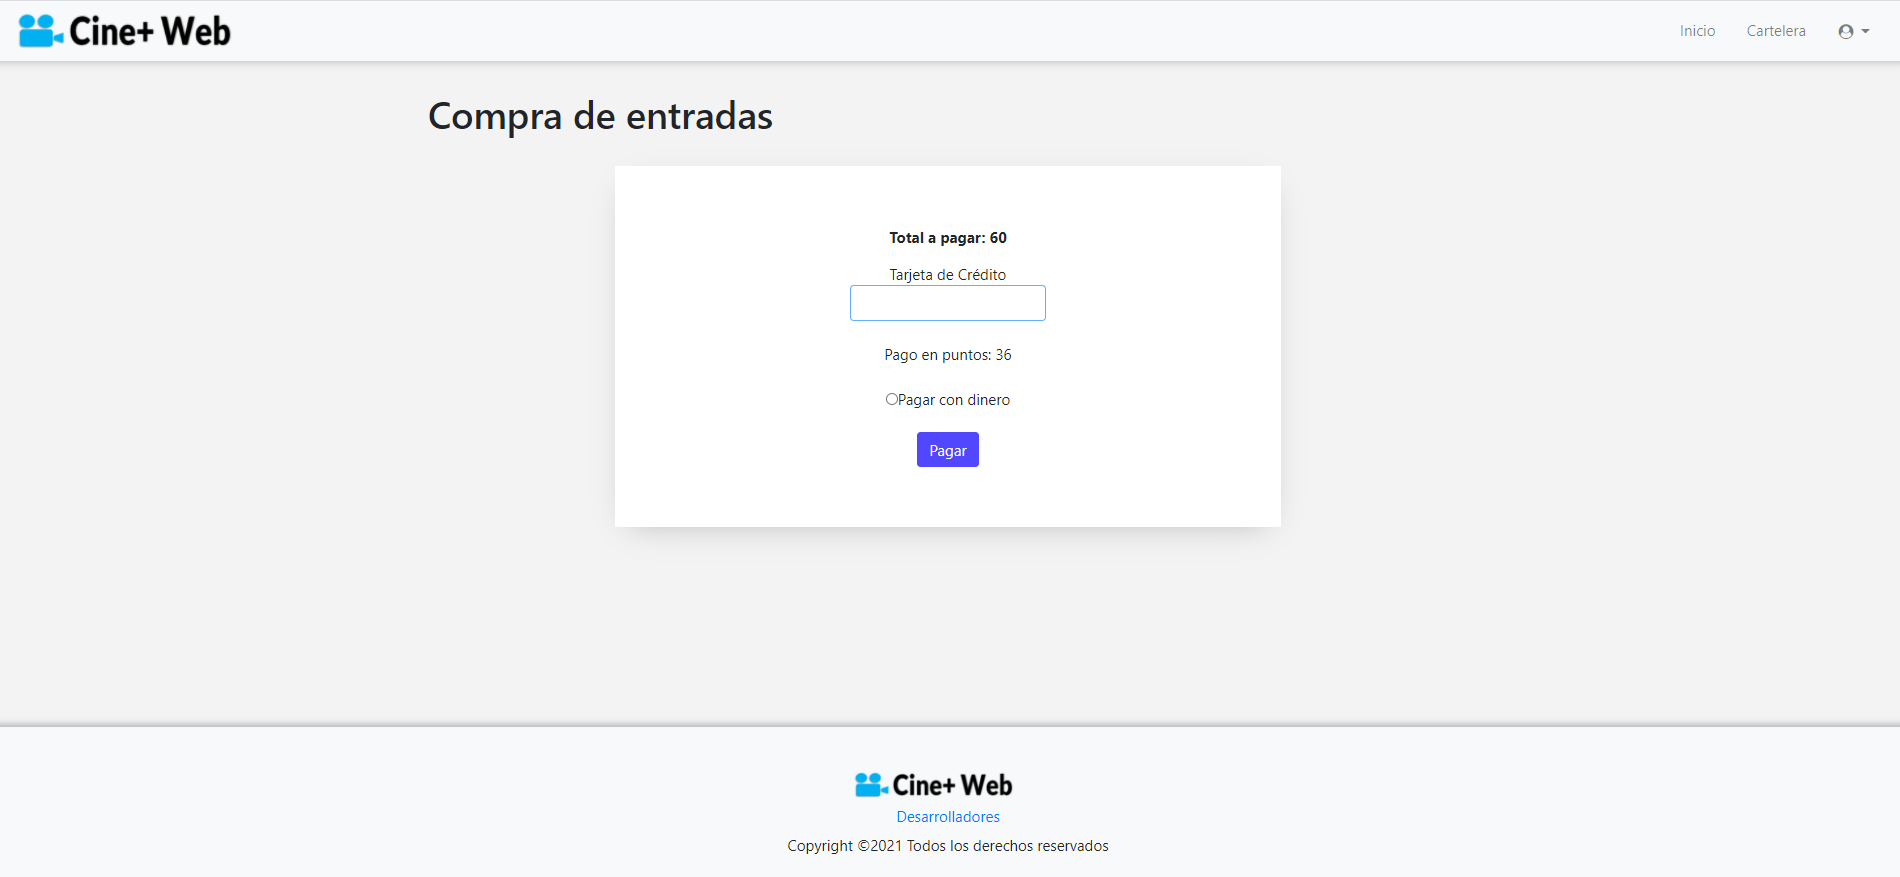
\includegraphics[scale=0.35]{./chapters/img/ticketpurchase2.png}
	
	\label{fig:ticketpurchase2}
	\caption{Tickect de compra}
	
\end{figure}


\subsubsection{Paso 5}
En este paso se muestra el c\'odigo de compra. El cliente debe guardarlo en caso que se desee cancelar la reservaci\'on

\begin{figure}[h!]
	\centering
	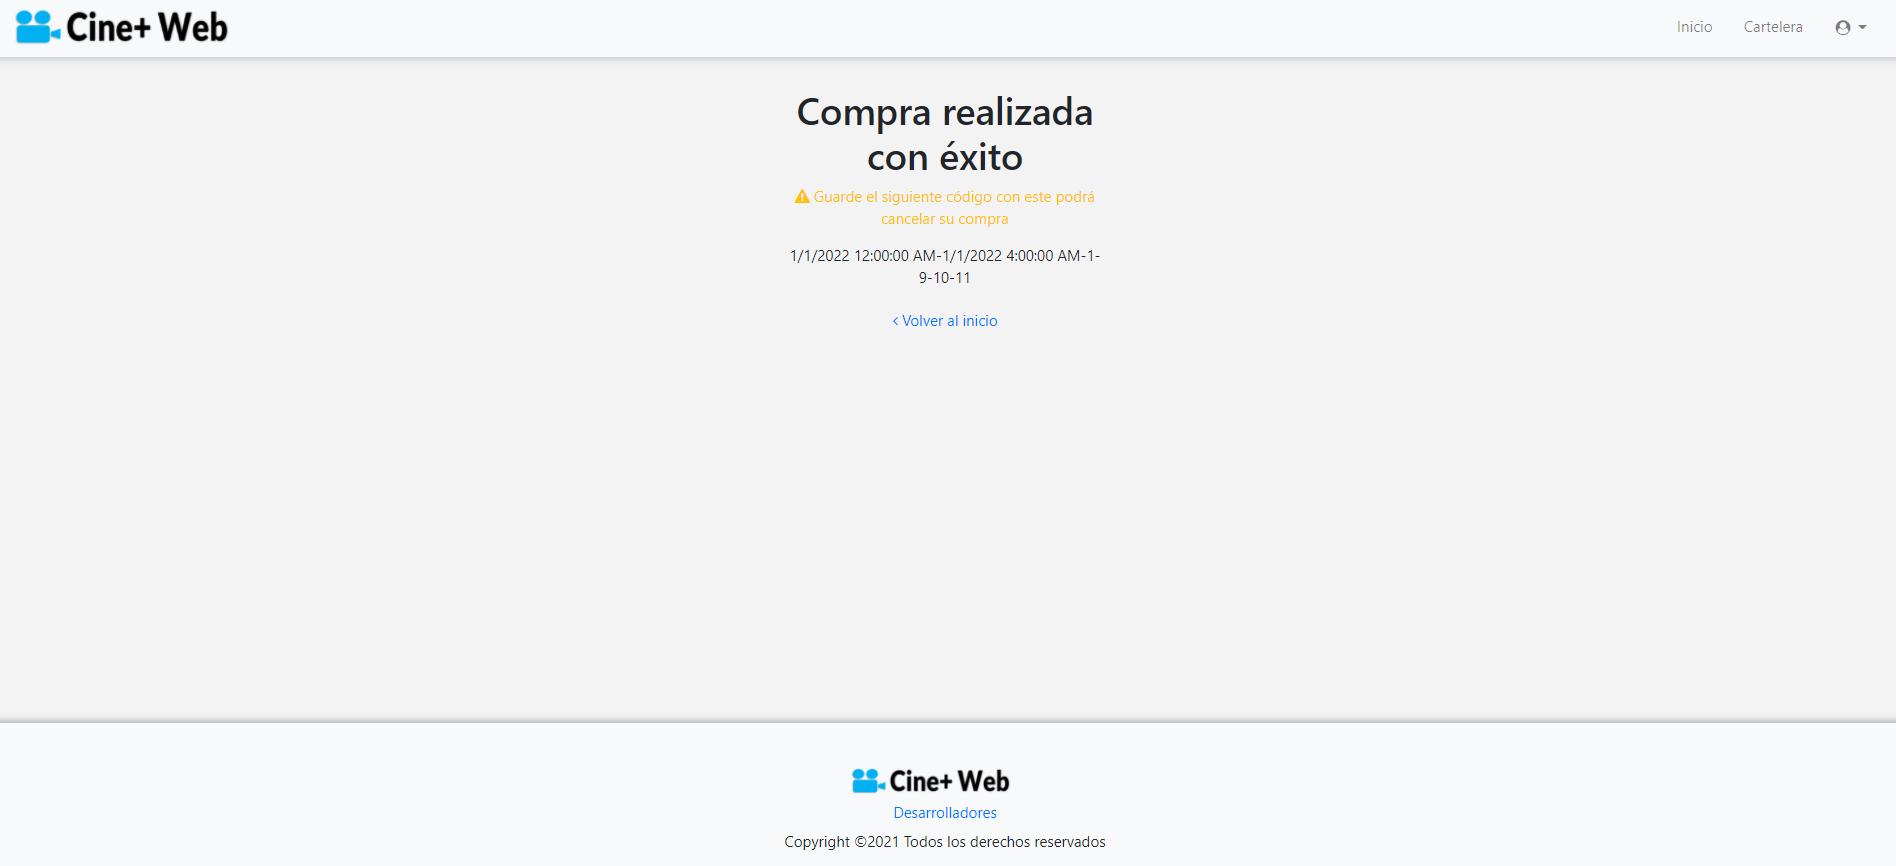
\includegraphics[scale=0.35]{./chapters/img/ticketpurchase3.png}
	
	\label{fig:ticketpurchase3}
	\caption{Tickect de compra}
	
\end{figure}

\subsection{Cancelaci\'on de compras}
Esta opci\'on se muestra junto a la opci\'on de compra en cada regl\'on de funciones, mediante un bot\'on que direcciona a una p\'agina donde se muestra el campo de c\'odigo de socio o tarjeta de cr\'edito y el c\'odigo de compra. EL primero de estos debe ser especificado en el caso de que el pago haya sido realizado por medio de una tarjeta de cr\'edito, especificar esta; o si se realiz\'o por los puntos de socio, especificar el c\'odigo del socio, el \'ultimo campo se debe rellenar con el c\'odigo mostrado en el ticket al efectuar la compra

\begin{figure}[h!]
	\centering
	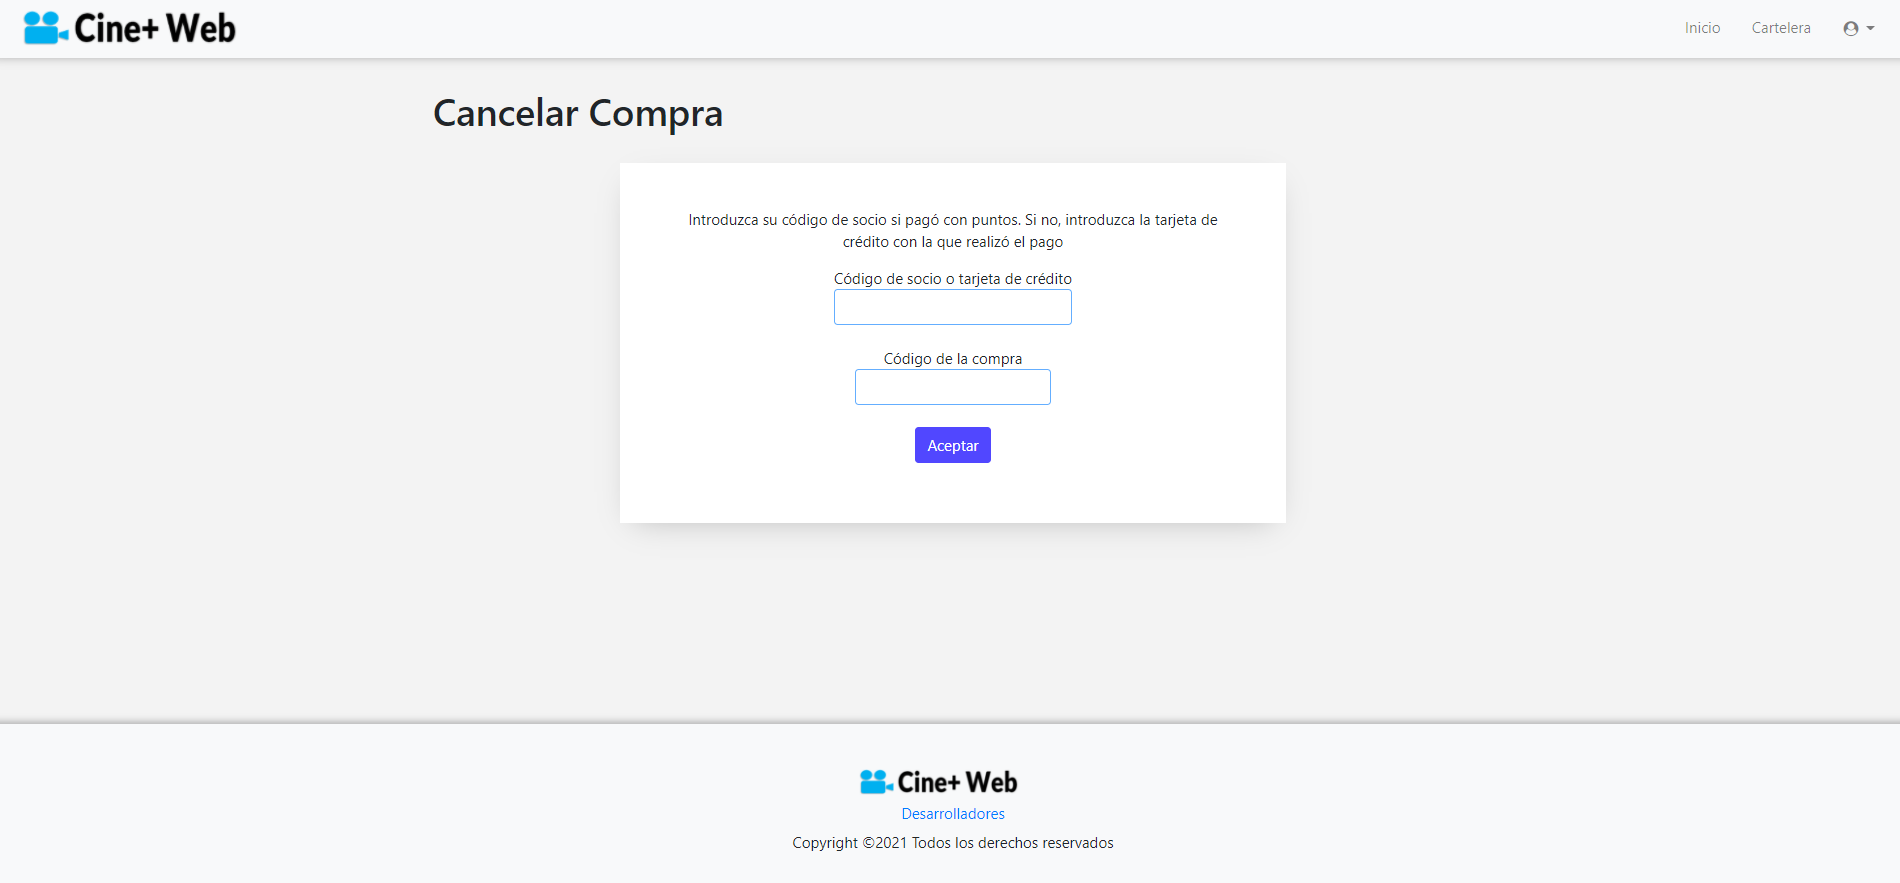
\includegraphics[scale=0.35]{./chapters/img/cancel.png}
	
	\label{fig:cancel}
	\caption{Cancelar compra}
	
\end{figure}
\subsection{Informaci\'on Personal}
El usuario puede visualizar su informaci\'on personal accediendo desde la pesta\~na con el \'icono de usuario, al hacer click en esta aparece la opci\'on Informaci\'on Personal, la que direcciona a una p\'agina donde se muestran los datos introducidos por el usuario en el registro de su cuenta adem\'as del c\'odigo de socio generado por el sistema.

\begin{figure}[h!]
	\centering
	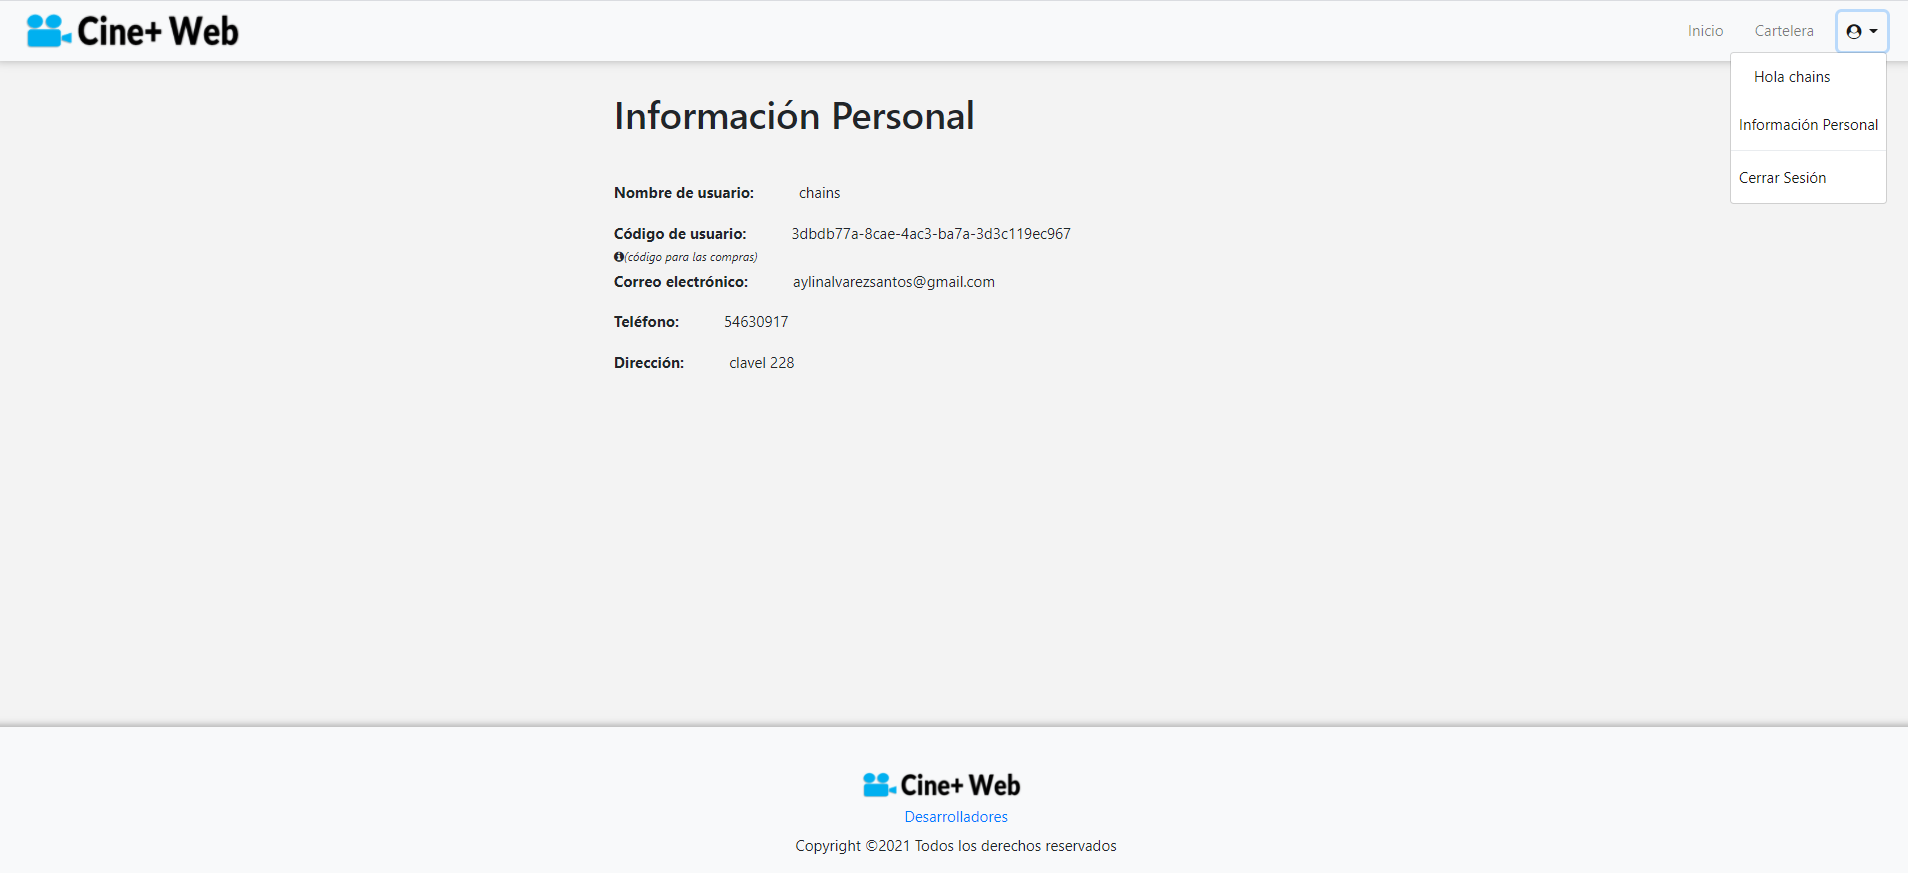
\includegraphics[scale=0.35]{./chapters/img/personal_info.png}
	
	\label{fig:personal_info}
	\caption{Informaci\'on Personal}
	
\end{figure}